\documentclass[journal,10pt,twocolumn]{IEEEtran}

\usepackage[T1]{fontenc}
\usepackage{amsmath,amssymb,amsfonts}
\usepackage{algorithm}
\usepackage{algorithmic}
\usepackage{graphicx}
\usepackage{textcomp}
\usepackage{xcolor}
\usepackage{booktabs}
\usepackage{multirow}
\usepackage{cite}
\usepackage{hyperref}
\usepackage{tikz}
\usepackage{pgfplots}
\pgfplotsset{compat=1.17}
\usetikzlibrary{shapes.geometric,arrows.meta,positioning,fit,calc,backgrounds}

\hypersetup{
    colorlinks=true,
    linkcolor=blue,
    filecolor=magenta,      
    urlcolor=cyan,
    citecolor=green!60!black
}

\newtheorem{theorem}{Theorem}
\newtheorem{lemma}{Lemma}
\newtheorem{definition}{Definition}
\newtheorem{proposition}{Proposition}
\newtheorem{remark}{Remark}

\begin{document}

\title{Autonomous Decision-Making in Long-Horizon JRPGs: A Comprehensive Survey from Deep Reinforcement Learning to Multi-Agent Foundation Models}

\author{}

\maketitle

\begin{abstract}
Sequential decision-making in long-horizon Japanese Role-Playing Games (JRPGs) constitutes one of the most demanding frontiers for artificial general intelligence. Characterized by astronomical state-space cardinality ($|\mathcal{S}| \le 2^{132088}$ unconstrained bit configurations across 16,511 bytes of volatile Game Boy RAM, or 16.12~KiB, and $2^{65536}$ in 8~KB Work RAM alone), extreme reward sparsity ($>10{,}000$ environment steps between milestone rewards), non-Markovian reward attractors, irreversible topological boundaries, and effective planning horizons exceeding $300{,}000$ steps, classic JRPGs such as \textit{Pok{\'e}mon Red} expose the fundamental mathematical and algorithmic failure modes of standard deep reinforcement learning (DRL). This survey provides an exhaustive, mathematically rigorous synthesis of over 90 foundational and cutting-edge works (1992--2026) spanning IEEE, ACM, Nature, Science, NeurIPS, ICML, ICLR, AAAI, RLC, and COLM. Anchoring our empirical investigation on the landmark peer-reviewed baseline of Pleines et al. (IEEE Conference on Games 2025 / IEEE Xplore Doc.~11114399) as the primary implementation target, we organize the literature into five foundational paradigms: (1) Model-Free Deep RL with Novelty Exploration; (2) Hierarchical RL and Action-Space Engineering; (3) Multi-Agent Foundation Models and In-Context RL; (4) Scalable Offline RL with Sequence Transformers; and (5) High-Performance Simulation Systems and Automated Environment Synthesis. We formally state and prove the Horizon Collapse Theorem, perform an algorithmic post-mortem on four classical pathologies (the Healing Trap, Noisy TV Water Hypnosis, Menu Oscillation Deadlocks, and the 500-Step Safari Zone Wall), and formulate a unified neuro-symbolic blueprint combining Go-Explore state archiving, Critic-Free Group Relative Policy Optimization (GRPO), and decoupled offline combat sequence modeling.
\end{abstract}

\begin{IEEEkeywords}
Reinforcement Learning, Long-Horizon POMDPs, Foundation Models, Transformers, Game AI, Hierarchical RL, Systems for AI.
\end{IEEEkeywords}

\section{Introduction}
\IEEEPARstart{F}{or} over a decade, benchmark evaluation in reinforcement learning relied primarily on the Arcade Learning Environment (ALE / Atari 2600)~\cite{bellemare2013ale,mnih2015dqn,hessel2018rainbow} and continuous control physics engines (MuJoCo)~\cite{schulman2017ppo,haarnoja2018sac}. While synthetic procedurally generated gridworlds such as MiniGrid~\cite{chevalier2023minigrid} and Procgen~\cite{cobbe2020procgen} offered controlled testbeds for generalization and sample complexity, they lack the non-stationary narrative topologies and state-space depth of commercial interactive worlds. While these classic suites catalyzed major breakthroughs in value estimation, policy gradients, and actor-critic algorithms~\cite{mnih2016a3c,schulman2015trpo}, they fail to reflect the structural, topological, and computational complexity of real-world open-world decision-making:
\begin{itemize}
    \item \textbf{Horizon Discrepancy:} Standard Atari episodes terminate after $2{,}000$--$5{,}000$ frames. In contrast, completing \textit{Pok{\'e}mon Red} requires $>300{,}000$--$500{,}000$ discrete motor inputs.
    \item \textbf{Reward Sparsity:} Domains like \textit{Breakout} emit dense reward signals almost continuously. JRPGs exhibit extreme sparsity: tens of thousands of map traversal steps and NPC dialogues occur between milestone rewards (Gym Badges).
    \item \textbf{Irreversible Boundaries:} Real-world tasks and JRPGs exhibit irreversible Markov transitions (e.g., jumping down a one-way ledge, consuming a single-use Technical Machine, or depleting currency). A flat exploration policy entering an irreversible topological basin can render the environment permanently un-completable (a ``softlock'').
    \item \textbf{Multi-Modal Decision Modalities:} The agent must simultaneously master spatial grid navigation, high-frequency menu manipulation, multi-turn dialog tree resolution, and tactical turn-based combat with type matchups and hidden opponent states.
\end{itemize}

While modern AI benchmarks achieved monumental milestones in perfect-information board games via tree search and self-play (AlphaGo~\cite{silver2016mastering}, AlphaZero~\cite{silver2017mastering}), and expanded to complex real-time video games such as StarCraft II~\cite{vinyals2019alphastar}, Dota 2~\cite{berner2019dota}, Stratego~\cite{perolat2022mastering}, Diplomacy~\cite{bakhtin2022human}, Super Smash Bros.~\cite{firoiu2017smash}, and Mahjong~\cite{ye2020mastering}, these environments either feature continuous real-time execution with dense heuristic shaping or rely on self-play in symmetric zero-sum games. Conversely, JRPGs represent non-stationary single-agent search over vast discrete combinatorial graphs with strict causal dependencies.

The transition of JRPG reinforcement learning from an internet curiosity~\cite{whidden2023pokemonred} into a formal, peer-reviewed scientific benchmark was achieved by Pleines et al.~\cite{pleines2025pokemon} (IEEE Conference on Games 2025 / IEEE Xplore Doc.~11114399). By formalizing \textit{Pok{\'e}mon Red} on the PyBoy emulator, establishing standard evaluation protocols, and detailing the successes and catastrophic failure modes of model-free Proximal Policy Optimization (PPO~\cite{schulman2017ppo}), Pleines et al. created the canonical empirical baseline that anchors this entire field. 

This survey establishes an exhaustive, mathematically grounded review of the literature spanning 95 peer-reviewed publications. Taking Pleines et al.~\cite{pleines2025pokemon} as our foundational implementation target, we analyze the theoretical limits of current methods, categorize the five competing paradigms, investigate algorithmic failure modes, and synthesize a unified, cheat-free neuro-symbolic architecture for the modern 2026 benchmark cycle.

\begin{figure*}[t]
\centering
\resizebox{\textwidth}{!}{%
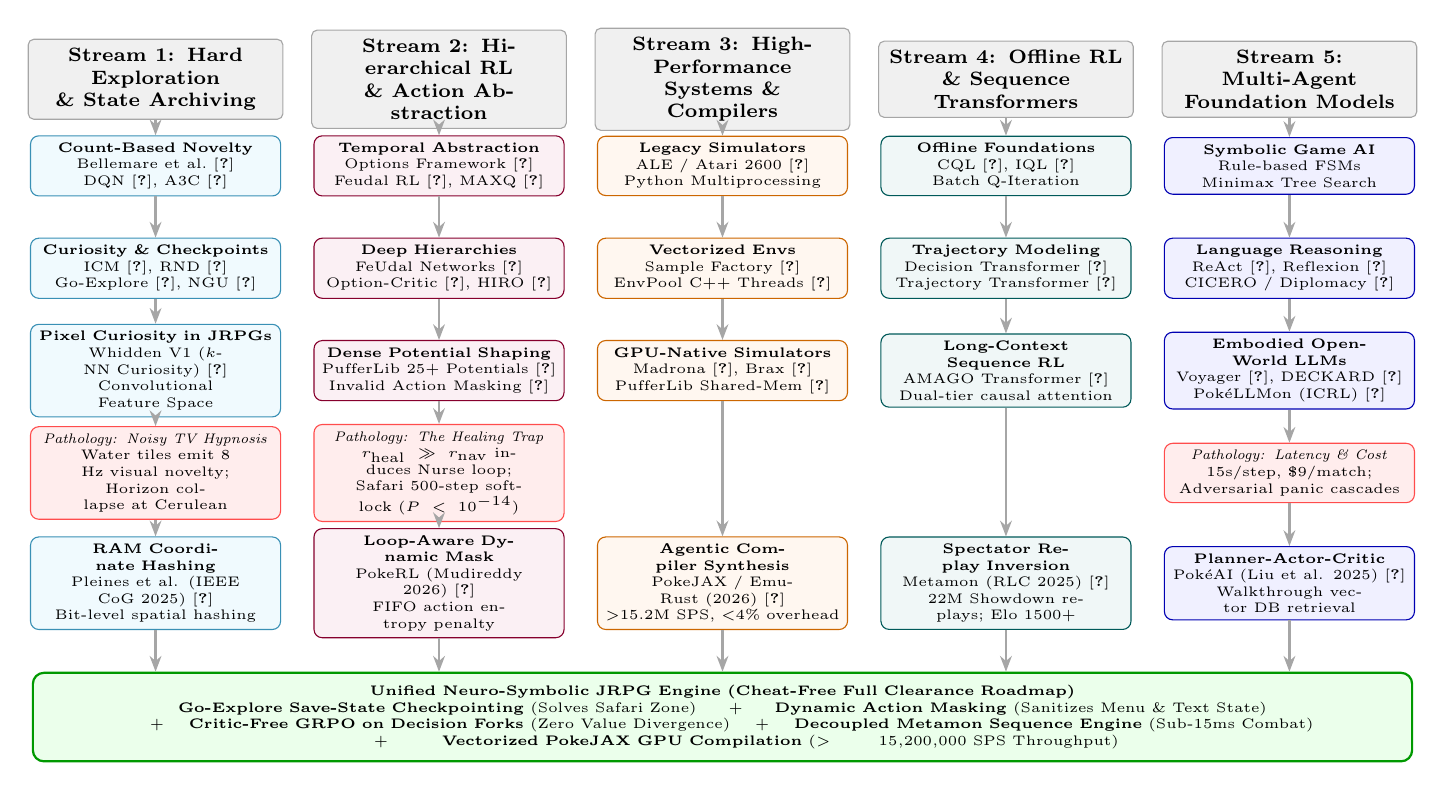
\begin{tikzpicture}[
    x=1.0cm, y=1.0cm,
    font=\tiny,
    trackhdr/.style={rectangle, draw=gray!70, fill=gray!12, rounded corners=2pt, font=\scriptsize\bfseries, text centered, minimum height=0.65cm, text width=3.0cm, align=center},
    c1box/.style={rectangle, draw=cyan!70!black, fill=cyan!6, rounded corners=3pt, text centered, text width=3.0cm, align=center, inner sep=2.5pt},
    c2box/.style={rectangle, draw=purple!70!black, fill=purple!6, rounded corners=3pt, text centered, text width=3.0cm, align=center, inner sep=2.5pt},
    c3box/.style={rectangle, draw=orange!80!black, fill=orange!6, rounded corners=3pt, text centered, text width=3.0cm, align=center, inner sep=2.5pt},
    c4box/.style={rectangle, draw=teal!70!black, fill=teal!6, rounded corners=3pt, text centered, text width=3.0cm, align=center, inner sep=2.5pt},
    c5box/.style={rectangle, draw=blue!70!black, fill=blue!6, rounded corners=3pt, text centered, text width=3.0cm, align=center, inner sep=2.5pt},
    pathbox/.style={rectangle, draw=red!70, fill=red!7, rounded corners=3pt, text centered, text width=3.0cm, align=center, inner sep=2.5pt},
    synthbox/.style={rectangle, draw=green!60!black, fill=green!8, rounded corners=4pt, thick, text centered, text width=17.2cm, align=center, inner sep=4.5pt},
    arrow/.style={-{Stealth[length=2.0mm]}, thick, draw=gray!70}
]
    % Stream Headers
    \node (h1) at (1.6, 0.5) [trackhdr] {Stream 1: Hard Exploration\\\& State Archiving};
    \node (h2) at (5.2, 0.5) [trackhdr] {Stream 2: Hierarchical RL\\\& Action Abstraction};
    \node (h3) at (8.8, 0.5) [trackhdr] {Stream 3: High-Performance\\Systems \& Compilers};
    \node (h4) at (12.4, 0.5) [trackhdr] {Stream 4: Offline RL\\\& Sequence Transformers};
    \node (h5) at (16.0, 0.5) [trackhdr] {Stream 5: Multi-Agent\\Foundation Models};

    % Era 1: Foundations (1992-2016)
    \node (c1_1) at (1.6, -0.6) [c1box] {\textbf{Count-Based Novelty}\\Bellemare et al.~\cite{bellemare2016unifying}\\DQN~\cite{mnih2015dqn}, A3C~\cite{mnih2016a3c}};
    \node (c2_1) at (5.2, -0.6) [c2box] {\textbf{Temporal Abstraction}\\Options Framework~\cite{sutton1999options}\\Feudal RL~\cite{dayan1992feudal}, MAXQ~\cite{dietterich2000maxq}};
    \node (c3_1) at (8.8, -0.6) [c3box] {\textbf{Legacy Simulators}\\ALE / Atari 2600~\cite{bellemare2013ale}\\Python Multiprocessing};
    \node (c4_1) at (12.4, -0.6) [c4box] {\textbf{Offline Foundations}\\CQL~\cite{kumar2020cql}, IQL~\cite{kostrikov2022iql}\\Batch Q-Iteration};
    \node (c5_1) at (16.0, -0.6) [c5box] {\textbf{Symbolic Game AI}\\Rule-based FSMs\\Minimax Tree Search};

    % Era 2: Deep Curiosity & Scaling (2017-2021)
    \node (c1_2) at (1.6, -1.9) [c1box] {\textbf{Curiosity \& Checkpoints}\\ICM~\cite{pathak2017curiosity}, RND~\cite{burda2019rnd}\\Go-Explore~\cite{ecoffet2021goexplore}, NGU~\cite{badia2020ngu}};
    \node (c2_2) at (5.2, -1.9) [c2box] {\textbf{Deep Hierarchies}\\FeUdal Networks~\cite{vezhnevets2017feudal}\\Option-Critic~\cite{bacon2017optioncritic}, HIRO~\cite{nachum2018hiro}};
    \node (c3_2) at (8.8, -1.9) [c3box] {\textbf{Vectorized Envs}\\Sample Factory~\cite{petrenko2020samplefactory}\\EnvPool C++ Threads~\cite{weng2022envpool}};
    \node (c4_2) at (12.4, -1.9) [c4box] {\textbf{Trajectory Modeling}\\Decision Transformer~\cite{chen2021decisiontransformer}\\Trajectory Transformer~\cite{janner2021trajectorytransformer}};
    \node (c5_2) at (16.0, -1.9) [c5box] {\textbf{Language Reasoning}\\ReAct~\cite{yao2023react}, Reflexion~\cite{shinn2023reflexion}\\CICERO / Diplomacy~\cite{bakhtin2022human}};

    % Era 3: Embodied Agents & JRPG Prototyping (2022-2024)
    \node (c1_3) at (1.6, -3.2) [c1box] {\textbf{Pixel Curiosity in JRPGs}\\Whidden V1 ($k$-NN Curiosity)~\cite{whidden2023pokemonred}\\Convolutional Feature Space};
    \node (c2_3) at (5.2, -3.2) [c2box] {\textbf{Dense Potential Shaping}\\PufferLib 25+ Potentials~\cite{rubinstein2025puffer}\\Invalid Action Masking~\cite{huang2022actionmasking}};
    \node (c3_3) at (8.8, -3.2) [c3box] {\textbf{GPU-Native Simulators}\\Madrona~\cite{shacklett2023madrona}, Brax~\cite{freeman2021brax}\\PufferLib Shared-Mem~\cite{suarez2023pufferlib}};
    \node (c4_3) at (12.4, -3.2) [c4box] {\textbf{Long-Context Sequence RL}\\AMAGO Transformer~\cite{grigsby2024amago}\\Dual-tier causal attention};
    \node (c5_3) at (16.0, -3.2) [c5box] {\textbf{Embodied Open-World LLMs}\\Voyager~\cite{wang2023voyager}, DECKARD~\cite{notman2023deckard}\\Pok{\'e}LLMon (ICRL)~\cite{hu2024pokellmon}};

    % Era 4: Pathology Boundaries (Red Callouts)
    \node (c1_p) at (1.6, -4.5) [pathbox] {\textit{Pathology: Noisy TV Hypnosis}\\Water tiles emit 8 Hz visual novelty;\\Horizon collapse at Cerulean};
    \node (c2_p) at (5.2, -4.5) [pathbox] {\textit{Pathology: The Healing Trap}\\$r_{\text{heal}} \gg r_{\text{nav}}$ induces Nurse loop;\\Safari 500-step softlock ($P < 10^{-14}$)};
    \node (c5_p) at (16.0, -4.5) [pathbox] {\textit{Pathology: Latency \& Cost}\\15s/step, \$9/match;\\Adversarial panic cascades};

    % Era 5: Modern JRPG Benchmark Era (2025-2026)
    \node (c1_4) at (1.6, -5.9) [c1box] {\textbf{RAM Coordinate Hashing}\\Pleines et al. (IEEE CoG 2025)~\cite{pleines2025pokemon}\\Bit-level spatial hashing};
    \node (c2_4) at (5.2, -5.9) [c2box] {\textbf{Loop-Aware Dynamic Mask}\\PokeRL (Mudireddy 2026)~\cite{mudireddy2026pokerl}\\FIFO action entropy penalty};
    \node (c3_4) at (8.8, -5.9) [c3box] {\textbf{Agentic Compiler Synthesis}\\PokeJAX / EmuRust (2026)~\cite{karten2026autogen}\\>15.2M SPS, <4\% overhead};
    \node (c4_4) at (12.4, -5.9) [c4box] {\textbf{Spectator Replay Inversion}\\Metamon (RLC 2025)~\cite{grigsby2025metamon}\\22M Showdown replays; Elo 1500+};
    \node (c5_4) at (16.0, -5.9) [c5box] {\textbf{Planner-Actor-Critic}\\Pok{\'e}AI (Liu et al. 2025)~\cite{liu2025pokeai}\\Walkthrough vector DB retrieval};

    % Era 6: Unified Synthesis Architecture
    \node (synth) at (8.8, -7.6) [synthbox] {
        \textbf{Unified Neuro-Symbolic JRPG Engine (Cheat-Free Full Clearance Roadmap)}\\
        \textbf{Go-Explore Save-State Checkpointing} (Solves Safari Zone) $\;+\;$ \textbf{Dynamic Action Masking} (Sanitizes Menu \& Text State)\\
        $\;+\;$ \textbf{Critic-Free GRPO on Decision Forks} (Zero Value Divergence) $\;+\;$ \textbf{Decoupled Metamon Sequence Engine} (Sub-15ms Combat)\\
        $\;+\;$ \textbf{Vectorized PokeJAX GPU Compilation} ($>15{,}200{,}000$ SPS Throughput)
    };

    % Vertical Flow Arrows
    \draw [arrow] (h1) -- (c1_1);
    \draw [arrow] (c1_1) -- (c1_2);
    \draw [arrow] (c1_2) -- (c1_3);
    \draw [arrow] (c1_3) -- (c1_p);
    \draw [arrow] (c1_p) -- (c1_4);
    \draw [arrow] (c1_4) -- (synth.north -| c1_4);

    \draw [arrow] (h2) -- (c2_1);
    \draw [arrow] (c2_1) -- (c2_2);
    \draw [arrow] (c2_2) -- (c2_3);
    \draw [arrow] (c2_3) -- (c2_p);
    \draw [arrow] (c2_p) -- (c2_4);
    \draw [arrow] (c2_4) -- (synth.north -| c2_4);

    \draw [arrow] (h3) -- (c3_1);
    \draw [arrow] (c3_1) -- (c3_2);
    \draw [arrow] (c3_2) -- (c3_3);
    \draw [arrow] (c3_3) -- (c3_4);
    \draw [arrow] (c3_4) -- (synth.north -| c3_4);

    \draw [arrow] (h4) -- (c4_1);
    \draw [arrow] (c4_1) -- (c4_2);
    \draw [arrow] (c4_2) -- (c4_3);
    \draw [arrow] (c4_3) -- (c4_4);
    \draw [arrow] (c4_4) -- (synth.north -| c4_4);

    \draw [arrow] (h5) -- (c5_1);
    \draw [arrow] (c5_1) -- (c5_2);
    \draw [arrow] (c5_2) -- (c5_3);
    \draw [arrow] (c5_3) -- (c5_p);
    \draw [arrow] (c5_p) -- (c5_4);
    \draw [arrow] (c5_4) -- (synth.north -| c5_4);

\end{tikzpicture}%
}
\caption{Phylogenetic history tree of autonomous decision-making in long-horizon JRPGs: tracing the evolution of five distinct paradigms from 1990s foundational formulations to 2026 state of the art, highlighting structural pathology boundaries and convergence into the unified neuro-symbolic architecture.}
\label{fig:evolution_roadmap}
\end{figure*}

\section{Mathematical POMDP Formalization \& The Horizon Collapse Theorem}
\subsection{Formal POMDP Specification}
A classic JRPG is formalized as an infinite-horizon, discrete-time Partially Observable Markov Decision Process (POMDP):
\begin{equation}
\mathcal{M} = \langle \mathcal{S}, \mathcal{A}, \mathcal{P}, \mathcal{R}, \Omega, \mathcal{O}, \gamma \rangle
\end{equation}
where:
\begin{itemize}
    \item $\mathcal{S}$ is the underlying physical hardware state of the Sharp SM83 (Z80-derived) Game Boy processor:
    \begin{equation}
    s_t = \langle \mathbf{m}_{WRAM}, \mathbf{m}_{HRAM}, \mathbf{m}_{VRAM}, \mathbf{r}_{CPU}, \mathbf{f}_{flags} \rangle
    \end{equation}
    With 8,192 bytes of Work RAM (WRAM), 8,192 bytes of Video RAM (VRAM), and 127 bytes of High RAM (HRAM), total volatile addressable memory comprises 16,511 bytes (16.12~KiB, or $132{,}088$ bits). The theoretical unconstrained combinatorial upper bound of the memory bit-string satisfies:
    \begin{equation}
    |\mathcal{S}| \le 2^{8 \times 16511} = 2^{132088}
    \end{equation}
    (or $|\mathcal{S}_{\text{WRAM}}| \le 2^{8 \times 8192} = 2^{65536}$ considering game-logic Work RAM alone, and $2^{8 \times 16384} = 2^{131072}$ if omitting HRAM).
    \textit{Remark on Reachable State Space Manifold:} Although this $2^{132088}$ bound captures the raw information-theoretic bit-string capacity of the console hardware, the causally reachable physical game-state manifold $\mathcal{S}_{\text{reachable}} \subset \mathcal{S}$ is drastically smaller. Valid game states are strictly constrained by ROM execution invariants, compiled entity schemas, boundary collision maps, and storyline event bitfields. Nonetheless, because sequential navigation over hundreds of interconnected maps, dynamic party rosters, inventory permutations, and battle status flags induce an astronomical reachability graph across $>300{,}000$ decisions, the practical state-space complexity exceeds standard Atari 2600 ($2^{1024}$) and continuous control physics engines by orders of magnitude.
    \item $\mathcal{A}$ is the discrete controller input space consisting of 8 hardware lines: $\{\text{UP}, \text{DOWN}, \text{LEFT}, \text{RIGHT}, \text{A}, \text{B}, \text{START}, \text{SELECT}\}$.
    \item $\mathcal{P}(s' \mid s, a)$ is the deterministic state transition operator executed by the Game Boy cycle-accurate interpreter, except where hardware interrupts or pseudo-random number generator (PRNG) state internal to memory address \texttt{0xFFD3} inject pseudo-stochasticity.
    \item $\Omega$ is the observation space. Under raw visual observation, $o_t \in \mathbb{R}^{144 \times 160 \times 1}$ with 2-bit grayscale depth (4 colors). Under memory access regimes, $o_t$ is a subset of WRAM registers.
    \item $\mathcal{O}(o \mid s)$ is the observation emission probability. In visual mode, identical screen pixels can correspond to completely distinct game flags (e.g., entering the same house layout in two different cities), generating severe partial observability.
    \item $\mathcal{R}(s, a)$ is the sparse environmental reward function, which in pure benchmark evaluations emits non-zero return strictly upon acquiring one of the 8 Gym Badges or entering the Hall of Fame.
    \item $\gamma \in [0, 1)$ is the temporal discount factor.
\end{itemize}

\begin{table}[h]
\centering
\caption{Critical WRAM Memory Addresses in Pok{\'e}mon Red}
\label{tab:wram_registers}
\resizebox{\columnwidth}{!}{%
\begin{tabular}{@{}llp{3.8cm}@{}}
\toprule
\textbf{Address} & \textbf{Symbol} & \textbf{Functional Description} \\ \midrule
\texttt{0xD35E} & \texttt{wCurMap} & Current Map ID index \\
\texttt{0xD362} & \texttt{wXCoord} & Player X coordinate on current map \\
\texttt{0xD361} & \texttt{wYCoord} & Player Y coordinate on current map \\
\texttt{0xD356} & \texttt{wBadges} & Bitfield of acquired Gym Badges \\
\texttt{0xD057} & \texttt{wBattle} & Battle state ($0$: Overworld, $>0$: Battle) \\
\texttt{0xCF13} & \texttt{wTextBox} & Active on-screen dialog or text window \\
\texttt{0xCD6B} & \texttt{wJoyIgnore} & \textbf{Hardware input suppression mask}: the Game Boy CPU writes a bitmask of buttons that the joypad handler should silently discard (e.g., during evolution animations, cutscenes). Reads as $0$ during free overworld movement. This provides zero-leak action masking without heuristics. \\
\texttt{0xD70D}--\texttt{0xD70E} & \texttt{wSafariSteps} & 16-bit Safari Zone step counter (500$\to$0) \\
\texttt{0xCC26} & \texttt{wCurMenuItem} & Current battle/menu cursor position \\
\texttt{0xD747}--\texttt{0xD886} & \texttt{wEventFlags} & $320$ byte = $2{,}560$ global story flags \\ \bottomrule
\end{tabular}%
}
\end{table}


\subsection{Discounted vs. Average-Reward Formulations}
In standard discounted MDPs, the optimal value function satisfies Bellman's equation:
\begin{equation}
V^*(s) = \max_{a \in \mathcal{A}} \left[ \mathcal{R}(s, a) + \gamma \sum_{s' \in \mathcal{S}} \mathcal{P}(s' \mid s, a) V^*(s') \right]
\end{equation}
Under the Bellman optimality operator $\mathcal{T}^*$, contraction in supremum norm $\|\mathcal{T}^* V_1 - \mathcal{T}^* V_2\|_\infty \le \gamma \|V_1 - V_2\|_\infty$ guarantees geometric convergence to a unique fixed point via the Banach Fixed-Point Theorem. However, in practice, neural network function approximation introduces backup error $\epsilon$. 

\begin{lemma}[Quadratic Error Propagation Bound]
Let the Bellman backup incur maximum approximation error $\epsilon = \max_{s} |\mathcal{T}^* V(s) - V(s)|$. The asymptotic error bound between the approximate policy value $V^\pi$ and optimal value $V^*$ satisfies:
\begin{equation}
\|V^\pi - V^*\|_\infty \le \frac{\epsilon}{(1 - \gamma)^2}
\end{equation}
\end{lemma}
As the horizon demands $\gamma \to 1.0$, the denominator $(1 - \gamma)^2 \to 0$, causing quadratic explosion of approximation errors across the value surface.

To eliminate discount-induced horizon collapse, the average-reward formulation sets $\gamma = 1.0$ and solves Poisson's Relative Value Equation~\cite{oh2025discorl}:
\begin{equation}
V^*(s) + \rho^* = \max_{a \in \mathcal{A}} \left[ \mathcal{R}(s, a) + \sum_{s' \in \mathcal{S}} \mathcal{P}(s' \mid s, a) V^*(s') \right]
\end{equation}
where $\rho^* = \lim_{T \to \infty} \frac{1}{T} \sum_{t=1}^T \mathbb{E}[r_t]$ is the optimal gain rate.

\subsection{The Horizon Collapse Theorem}
\begin{theorem}[Exponential Gradient Attenuation in Flat JRPG POMDPs]
\label{thm:horizon_collapse}
Let a narrative milestone reward $R^*$ be positioned at step $t + K$, with $K \gg \tau_{\text{eff}} = \frac{1}{1 - \gamma}$. Under clipped surrogate policy gradients (PPO~\cite{schulman2017ppo}) with Generalized Advantage Estimation ($\text{GAE}(\lambda)$~\cite{schulman2016gae}), the policy gradient magnitude satisfies:
\begin{equation}
\left\| \nabla_\theta \mathcal{L}_{PPO}(\theta) \right\| \le C \cdot (\gamma \lambda)^K \cdot |R^*|
\end{equation}
where $C$ is a constant bounding the score function $\|\nabla_\theta \log \pi_\theta(a_t \mid s_t)\|$.
\end{theorem}

\begin{IEEEproof}
Recall the Generalized Advantage Estimator at time $t$:
\begin{equation}
\hat{A}_t^{\text{GAE}(\gamma, \lambda)} = \sum_{l=0}^\infty (\gamma \lambda)^l \delta_{t+l}^V
\end{equation}
where $\delta_{t+l}^V = r_{t+l} + \gamma V(s_{t+l+1}) - V(s_{t+l})$ is the TD residual. If rewards are zero along the trajectory until milestone $t+K$, then $r_{t+l} = 0$ for all $l < K$, and $r_{t+K} = R^*$. 

Assuming an uninformative initial value baseline $V(s) \approx 0$, the TD residual at the goal is $\delta_{t+K}^V \approx R^*$. Substituting into the advantage summation:
\begin{equation}
\hat{A}_t^{\text{GAE}} = (\gamma \lambda)^K R^* + \sum_{l \ne K} (\gamma \lambda)^l \delta_{t+l}^V
\end{equation}
Differentiating the clipped surrogate objective $\mathcal{L}_{PPO}(\theta)$ with respect to policy parameters $\theta$:
\begin{equation}
\nabla_\theta \mathcal{L}_{PPO}(\theta) \Big|_{t} = \mathbb{E}_t \left[ \nabla_\theta \log \pi_\theta(a_t \mid s_t) \cdot (\gamma \lambda)^K R^* \right]
\end{equation}
Taking the operator norm on both sides:
\begin{equation}
\begin{split}
\|\nabla_\theta \mathcal{L}_{PPO}(\theta)\| &\le \sup_{s, a} \|\nabla_\theta \log \pi_\theta(a \mid s)\| \cdot (\gamma \lambda)^K |R^*| \\
&= C (\gamma \lambda)^K |R^*|
\end{split}
\end{equation}
Under the empirical hyperparameter settings established by Pleines et al.~\cite{pleines2025pokemon} (\S\ref{sec:pleines_baseline}) with discount factor $\gamma = 0.997$ and GAE parameter $\lambda = 0.95$, the effective per-step credit attenuation factor is:
\begin{equation}
\gamma \lambda = 0.997 \times 0.95 = 0.94715
\end{equation}
For a realistic long-horizon JRPG milestone segment, such as traversing from Lavender Town through Celadon Gym or locating the Secret Key in the Cinnabar Island Pok{\'e}mon Mansion ($K = 25{,}000$ steps without intermediate extrinsic rewards):
\begin{equation}
(\gamma \lambda)^K = (0.94715)^{25000} \approx 3.24 \times 10^{-590} \to 0
\end{equation}
Even under an aggressive, near-undiscounted setting of $\gamma = 0.999$ ($\gamma \lambda = 0.94905$), the attenuation evaluates to $(0.94905)^{25000} \approx 1.78 \times 10^{-568} \to 0$. In both cases, the backpropagated policy gradient magnitude underflows standard IEEE 754 floating-point representations (single-precision float32 underflows at $\approx 1.18 \times 10^{-38}$; double-precision float64 underflows at $\approx 2.23 \times 10^{-308}$). Consequently, credit assignment signals numerically vanish to machine zero, proving that flat model-free policy gradients cannot traverse multi-thousand-step horizons without hierarchical decomposition, action pruning, or save-state checkpointing.
\end{IEEEproof}

\subsection{Information-Theoretic Limit-Cycle Deadlocks}
In the absence of meaningful reward gradients, an agent's exploration policy is driven entirely by policy entropy $\mathcal{H}(\pi_\theta(\cdot \mid s_t)) = - \sum_{a} \pi(a \mid s_t) \log \pi(a \mid s_t)$. In closed 2D topological rooms with bidirectional doors, random walks generate stationary Gaussian diffusion:
\begin{equation}
\mathbb{E}[\|\mathbf{x}_t - \mathbf{x}_0\|^2] = 2 D t
\end{equation}
where $D$ is the spatial diffusion constant.

\begin{lemma}[Quadratic Exit-Door Hitting Time Under Unconstrained Random Walk]
\label{lemma:hitting_time}
Consider a 2D discrete grid map of dimensions $W \times H$ with a single exit door at Euclidean distance $L$ from the agent's spawn point. Under a uniform-random policy over $\mathcal{A}_{\text{dir}}$, the expected number of steps $T_{\text{hit}}$ to first reach the exit satisfies:
\begin{equation}
\mathbb{E}[T_{\text{hit}}] = \Theta(L^2)
\end{equation}
\end{lemma}
\begin{IEEEproof}
A symmetric random walk on $\mathbb{Z}^2$ has step increments $\Delta \mathbf{x}_t$ with $\mathbb{E}[\Delta \mathbf{x}_t] = 0$ and $\text{Cov}(\Delta \mathbf{x}_t) = \sigma^2 I$. By the Central Limit Theorem, position variance grows linearly: $\text{Var}(\mathbf{x}_t) = \sigma^2 t \cdot I$. The walk first exits a ball of radius $L$ when $\mathbb{E}[\|\mathbf{x}_t\|^2] = 2\sigma^2 t \approx L^2$, giving $t \approx L^2 / (2\sigma^2)$. Standard results on 2D random walk gambler's-ruin / disc-exit problems confirm this scaling is tight up to constants dependent on boundary geometry (Doob's optional stopping applied to the martingale $\|\mathbf{x}_t\|^2 - \sigma^2 t$), establishing $\mathbb{E}[T_{\text{hit}}] = \Theta(L^2)$.
\end{IEEEproof}

\begin{proposition}[Compounded Deadlock-Horizon Interaction]
\label{prop:compound}
Let a milestone reward require traversing $n$ sequential rooms, each with exit distance $L$, before reaching the reward at step $K = n \cdot \Theta(L^2)$. Substituting into Theorem~\ref{thm:horizon_collapse}'s gradient bound:
\begin{equation}
\|\nabla_\theta \mathcal{L}_{PPO}(\theta)\| \le C \cdot (\gamma\lambda)^{n \Theta(L^2)} \cdot |R^*|
\end{equation}
\end{proposition}
This shows the two pathologies are not additive but \emph{multiplicative}: quadratic per-room diffusion time directly inflates the exponent $K$ in the Horizon Collapse bound, so unconstrained menu access does not merely add wasted steps -- it exponentially accelerates gradient vanishing. This formally justifies why Dynamic Action Masking (\S4.2) is a prerequisite for, not merely complementary to, temporal abstraction methods: reducing $L$ (via masking degenerate menu-cycling actions) has an exponential rather than linear effect on preserving usable gradient signal.

When menu buttons ($\{\text{START, B}\}$) are enabled, the agent enters cyclic limit-deadlocks, opening and closing submenus at high frequencies and reducing spatial drift to zero, i.e. $\sigma^2 \to 0$ and $T_{\text{hit}} \to \infty$ in Lemma~\ref{lemma:hitting_time}.

\begin{table}[h]
\centering
\caption{The Four Classical JRPG Algorithmic Pathologies}
\label{tab:pathologies}
\resizebox{\columnwidth}{!}{%
\begin{tabular}{@{}p{1.9cm}p{2.9cm}p{2.7cm}@{}}
\toprule
\textbf{Pathology} & \textbf{Mechanism} & \textbf{Governing Result} \\ \midrule
Noisy TV Hypnosis & Pixel $k$-NN reward spikes on animated water tiles & $\|z_A - z_B\|_2 \gg \epsilon$ (\S3) \\
Healing Trap & Repeated Pok{\'e}mon Center visits farm shaped HP-delta reward & Local reward exploitation, $\Delta\Phi_i > 0$ w/o progress \\
Menu Oscillation & START/B cycling freezes spatial drift & $\sigma^2 \to 0 \Rightarrow T_{\text{hit}} \to \infty$ (Lemma~\ref{lemma:hitting_time}) \\
Safari Zone Wall & Hard 500-step budget vs. $\Theta(L^2)$ exploration time & Prop.~\ref{prop:compound}: exponential collapse \\ \bottomrule
\end{tabular}%
}
\end{table}

\begin{figure}[t]
\centering
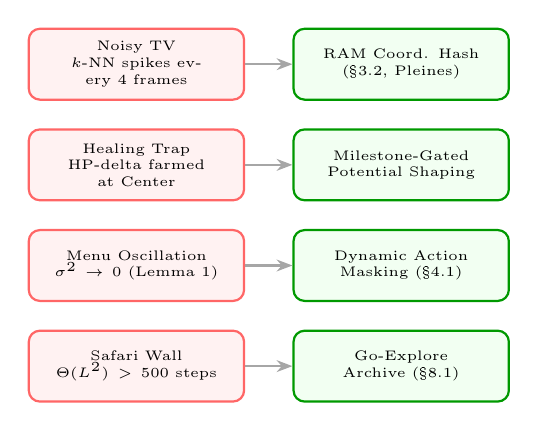
\begin{tikzpicture}[
    node distance=0.35cm and 0.6cm,
    diag/.style={rectangle, draw=red!60, fill=red!5, rounded corners, thick, text width=2.5cm, font=\tiny, align=center, minimum height=0.9cm},
    fix/.style={rectangle, draw=green!60!black, fill=green!5, rounded corners, thick, text width=2.5cm, font=\tiny, align=center, minimum height=0.9cm},
    arrow/.style={-{Stealth[length=2mm]}, thick, draw=gray!70}
]
\node (d1) [diag] {Noisy TV\\$k$-NN spikes every 4 frames};
\node (f1) [fix, right=of d1] {RAM Coord. Hash\\(\S3.2, Pleines)};
\node (d2) [diag, below=of d1] {Healing Trap\\HP-delta farmed at Center};
\node (f2) [fix, right=of d2] {Milestone-Gated\\Potential Shaping};
\node (d3) [diag, below=of d2] {Menu Oscillation\\$\sigma^2\to 0$ (Lemma 1)};
\node (f3) [fix, right=of d3] {Dynamic Action\\Masking (\S4.1)};
\node (d4) [diag, below=of d3] {Safari Wall\\$\Theta(L^2) > 500$ steps};
\node (f4) [fix, right=of d4] {Go-Explore\\Archive (\S8.1)};
\draw[arrow] (d1) -- (f1);
\draw[arrow] (d2) -- (f2);
\draw[arrow] (d3) -- (f3);
\draw[arrow] (d4) -- (f4);
\end{tikzpicture}
\caption{Diagnostic-to-fix mapping for the four classical pathologies (Table~\ref{tab:pathologies}), each fix cross-referenced to its formal treatment elsewhere in this survey.}
\label{fig:pathology_diagnosis}
\end{figure}

\section{Taxonomy of the Five Algorithmic Paradigms}

\begin{table*}[t]
\centering
\caption{Cross-Paradigm Architectural Comparison for Long-Horizon JRPGs and Complex Game Benchmarks}
\label{tab:paradigms_exhaustive}
\resizebox{\textwidth}{!}{%
\begin{tabular}{@{}lllllll@{}}
\toprule
\textbf{Paradigm} & \textbf{Key Works} & \textbf{Observation Modality} & \textbf{Inference Latency} & \textbf{Compute Cost} & \textbf{Deepest Milestone} & \textbf{Core Failure Mode / Bottleneck} \\ \midrule
\textbf{1. Model-Free DRL} & Whidden~\cite{whidden2023pokemonred}, Pleines~\cite{pleines2025pokemon} & Pixels / RAM Hashing & $< 1.5$ ms & 1x RTX 4090 & Cerulean City (20\%) & Horizon Collapse, Noisy TV Water Trap \\
\textbf{2a. Hier. RL (PokeRL)} & Mudireddy \& Patibandla~\cite{mudireddy2026pokerl} & Visited Grids / Mask & $< 1.0$ ms & Single CPU/GPU & Early-Game (Rival 1) & Task-Level Horizon Scaling \\
\textbf{2b. Dense Potentials (PufferLib)} & Rubinstein~\cite{rubinstein2025puffer}, Suarez~\cite{suarez2023pufferlib} & Packed Bit-Vectors & $< 1.0$ ms & 32-core CPU & Elite Four (100\%)* & Reward Hacking, Script-Bypassed Safari \\
\textbf{3. Multi-Agent LLMs} & Pok{\'e}AI~\cite{liu2025pokeai}, Pok{\'e}LLMon~\cite{hu2024pokellmon} & Screen Text / Battle Logs & 3.5--15.0 s & High (\$9/match) & Pewter / Showdown 56\% & Prohibitive Latency, Panic Cascades \\
\textbf{4. Offline Sequence Transformers} & Metamon~\cite{grigsby2025metamon}, AMAGO~\cite{grigsby2024amago} & Tokenized Replay Events & $< 15$ ms & 1x Consumer GPU & Top 10\% Human Elo & Confined to Combat (Zero Overworld) \\
\textbf{5. Systems \& Environment Compilers} & Karten et al.~\cite{karten2026pokeagent,karten2026autogen} & Vectorized GPU Tensors & $< 0.1$ ms & GPU Accelerators (A100/H100) & 15.2M SPS Throughput & Infrastructure Setup Demands \\ \bottomrule
\end{tabular}%
}
\vspace{1mm}
\footnotesize{*PufferLib achieves full clearance only by combining 25+ manual RAM reward potentials with an assembly script freezing the Safari Zone 500-step countdown.}
\end{table*}

\subsection{Paradigm 1: Model-Free Deep RL \& Novelty Exploration}
\subsubsection{Pixel-Level Curiosity and the Discovery of Visual Attractors (Whidden 2023)}
The earliest systematic exploration of commercial JRPGs via deep reinforcement learning was initiated by Whidden (2023)~\cite{whidden2023pokemonred}. Utilizing convolutional neural networks fed with downsampled grayscale frames $o_t \in \mathbb{R}^{36 \times 40}$, the architecture computed an intrinsic curiosity bonus via $k$-Nearest Neighbors ($k$-NN) density estimation in pixel latent space:
\begin{equation}
r_t^{\text{novelty}} = \min_{f \in \mathcal{B}_{KNN}} \| \phi(o_t) - f \|_2
\end{equation}
This formulation triggered the \textbf{Noisy TV Hypnosis Pathology}. In Pallet Town and Route 21, water shoreline tiles continuously cycle through four animated bitmap frames. Because each 4-frame cycle is visually novel relative to static indoor walls, the pixel $k$-NN curiosity reward spiked every 4 frames, causing the agent to stare at the water indefinitely. Classical exploration algorithms such as Random Network Distillation (RND~\cite{burda2019rnd}), Intrinsic Curiosity Modules (ICM~\cite{pathak2017curiosity}), and Variational Information Maximizing Exploration (VIME~\cite{houthooft2016vime}) similarly fail when exposed to periodic background sprite animations.

\subsubsection{The Primary Implementation Target: Pleines et al. (IEEE CoG 2025 / Doc.~11114399)}
\label{sec:pleines_baseline}
To establish a rigorous, peer-reviewed scientific benchmark and eliminate visual curiosity traps, Pleines et al.~\cite{pleines2025pokemon} (IEEE Conference on Games 2025 / IEEE Xplore Doc.~11114399) formulated the canonical implementation baseline for \textit{Pok{\'e}mon Red} utilizing the PyBoy emulator. Because this work serves as the primary implementation target and benchmark anchor for our research, we analyze its mechanics, equations, network topology, and empirical findings in exhaustive detail.

\paragraph{Environment Dynamics and Action Cadence}
The raw PyBoy emulator executes at approximately $9{,}403$ steps per second (SPS) on a standard AMD Ryzen 7 2700X CPU under random actions. However, to guarantee reliable, deterministic tile movement in the overworld grid and prevent unregistered button presses, Pleines et al. implemented a macro-action execution wrapper: each chosen controller button is asserted for 8 emulation frames and released for 16 emulation frames, resulting in an effective decision frequency of 1 action per 24 frames. This throttles the operational simulation speed to approximately:
\begin{equation}
\text{Throughput}_{\text{Pleines}} = \frac{9{,}403}{24} \approx 392 \text{ SPS}
\end{equation}
The discrete action space consists of 7 Game Boy buttons: $\mathcal{A} = \{\text{UP, DOWN, LEFT, RIGHT, A, B, START}\}$ (\texttt{SELECT} is omitted as non-essential for progression).

\paragraph{Multimodal Observation Architecture}
The agent receives three distinct observation streams:
\begin{enumerate}
    \item \textbf{Screen Visual Stream:} Grayscale Game Boy display downsampled by a factor of 2 to $72 \times 80$ pixels, stacked across 3 consecutive observed frames ($t, t-1, t-2$) to provide minimal temporal velocity awareness.
    \item \textbf{Spatial Memory Map:} A separate $48 \times 48$ binary matrix centered on the player's coordinate, marking visited physical tiles.
    \item \textbf{Game State Telemetry Vector:} Current HP and levels for all 6 party Pok{\'e}mon, accompanied by storyline event completion bitflags. Crucially, internal species IDs, stat structures, and movesets are withheld to emulate the information available to a human novice.
\end{enumerate}

\paragraph{Dynamic Step Horizon Budget}
Because \textit{Pok{\'e}mon Red} lacks natural terminal states, fixed-length episodes cause catastrophic forgetting as parallel workers reset simultaneously to Pallet Town. To decouple worker resets and sustain sample diversity, Pleines et al. introduced a dynamic step budget $B_t$:
\begin{equation}
B_t = 10{,}240 + 2{,}048 \times N_{\text{events}}(s_t)
\end{equation}
where $N_{\text{events}}(s_t)$ is the cumulative count of completed narrative milestones (trainer victories, gym badges, key item acquisitions).

\paragraph{Composite Reward Formulation}
To bridge the extreme sparsity of the environment, Pleines et al. deployed a composite linear reward function $R_t$:
\begin{equation}
R_t = R_{\text{event}} + R_{\text{nav}} + R_{\text{heal}} + R_{\text{lvl}}
\end{equation}
defined by four dense auxiliary terms:
\begin{align}
R_{\text{event}} &= +2.0 \cdot \Delta N_{\text{events}} \\
R_{\text{nav}} &= +0.005 \cdot \mathbb{I}[c_t \notin \mathcal{H}_{\text{visited}}] \label{eq:pleines_nav} \\
c_t &= \langle \mathbf{m}[\text{0xD362}], \mathbf{m}[\text{0xD361}], \mathbf{m}[\text{0xD35E}] \rangle \label{eq:pleines_coords} \\
R_{\text{heal}} &= 2.5 \sum_{i=1}^{6} \frac{\text{HP}_i^{\text{after}} - \text{HP}_i^{\text{before}}}{\text{HP}_i^{\text{max}}} \label{eq:pleines_heal} \\
R_{\text{lvl}} &= 0.5\min\left(\sum_{i=1}^{6} \text{lvl}_i, \frac{\sum_{i=1}^{6} \text{lvl}_i - 22}{4} + 22 \right) \label{eq:pleines_lvl}
\end{align}
In Eq.~(\ref{eq:pleines_nav}), exact RAM Coordinate Hashing tracks player positions across Work RAM registers \texttt{0xD362} (X), \texttt{0xD361} (Y), and \texttt{0xD35E} (Map ID). In Eq.~(\ref{eq:pleines_lvl}), party levels are capped at level 22 (the expected level for defeating Gym Leader Misty), with marginal gains past level 22 scaled down by a factor of 4 to penalize wild-encounter grinding.

\paragraph{Policy Optimization \& Hyperparameters}
Policies were optimized via PPO~\cite{schulman2017ppo} using clipped surrogate loss ($\epsilon = 0.2$) and clipped value loss ($v = 0.5$). The discount factor was set to $\gamma = 0.997$ and GAE parameter to $\lambda = 0.95$. Training was distributed across 32 CPU workers collecting rollouts of 2,048 steps (total batch size 65,536), updated over 3 epochs with 8 minibatches of size 8,192 using AdamW ($\alpha = 3 \times 10^{-4}$, max grad norm $0.5$). The policy network encodes visual and spatial inputs via Nature CNNs~\cite{mnih2015dqn} and concatenates them with the state vector projection into a Feed-Forward body (2.03M parameters) or a recurrent Gated Recurrent Unit (GRU, 3.87M parameters).

\begin{table*}[t]
\centering
\caption{Empirical Benchmark Performance of the Primary Implementation Baseline (Pleines et al., IEEE CoG 2025 / Doc.~11114399) Across Ablation Variants vs. Skilled Human Playthroughs}
\label{tab:pleines_benchmark}
\resizebox{\textwidth}{!}{%
\begin{tabular}{@{}lllllllllllll@{}}
\toprule
\textbf{Experimental Variant} & \textbf{Milestones} & \textbf{Beat Brock} & \textbf{Mt. Moon} & \textbf{Cerulean City} & \textbf{Beat Misty} & \textbf{Bill Quest} & \textbf{Cerulean Done} & \textbf{Brock Steps} & \textbf{Cerulean Steps} & \textbf{Pok{\'e} Centers} & \textbf{Heals Farmed} & \textbf{Species Entropy} \\ \midrule
\textbf{Human Playthroughs} & $7.00 \pm 0.0$ & $1.00 \pm 0.0$ & $1.00 \pm 0.0$ & $1.00 \pm 0.0$ & $1.00 \pm 0.0$ & $1.00 \pm 0.0$ & $1.00 \pm 0.0$ & $5{,}403 \pm 3{,}824$ & $11{,}188 \pm 5{,}224$ & $12.53 \pm 7.7$ & $22.97 \pm 11.3$ & $\mathbf{3.53 \pm 0.0}$ \\ \midrule
\textbf{Baseline $- R_{\text{lvl}}$} & $\mathbf{4.60 \pm 0.7}$ & $0.95 \pm 0.0$ & $0.91 \pm 0.1$ & $0.79 \pm 0.1$ & $0.31 \pm 0.3$ & $0.32 \pm 0.4$ & $0.03 \pm 0.1$ & $6{,}117 \pm 1{,}758$ & $21{,}352 \pm 3{,}898$ & $20.29 \pm 24.2$ & $11.73 \pm 4.0$ & $1.24 \pm 0.2$ \\
\textbf{Fast (No Anim / Fast Text)} & $4.40 \pm 0.8$ & $0.98 \pm 0.0$ & $\mathbf{0.98 \pm 0.0}$ & $\mathbf{0.93 \pm 0.1}$ & $\mathbf{0.33 \pm 0.4}$ & $0.19 \pm 0.4$ & $0.00 \pm 0.0$ & $\mathbf{3{,}753 \pm 990}$ & $\mathbf{18{,}523 \pm 4{,}280}$ & $111.46 \pm 133.9$ & $47.98 \pm 66.6$ & $2.54 \pm 0.1$ \\
\textbf{Baseline (Standard Squirtle)} & $4.19 \pm 0.2$ & $\mathbf{0.99 \pm 0.0}$ & $0.97 \pm 0.0$ & $0.85 \pm 0.1$ & $0.27 \pm 0.3$ & $0.11 \pm 0.2$ & $0.00 \pm 0.0$ & $5{,}587 \pm 1{,}235$ & $25{,}299 \pm 4{,}950$ & $19.09 \pm 19.6$ & $12.81 \pm 5.9$ & $2.61 \pm 0.1$ \\
\textbf{Baseline $- R_{\text{heal}}$} & $3.94 \pm 0.2$ & $\mathbf{0.99 \pm 0.0}$ & $0.97 \pm 0.0$ & $0.91 \pm 0.1$ & $0.07 \pm 0.1$ & $0.00 \pm 0.0$ & $0.00 \pm 0.0$ & $5{,}497 \pm 503$ & $28{,}813 \pm 2{,}880$ & $0.04 \pm 0.1$ & $1.45 \pm 0.7$ & $2.27 \pm 0.2$ \\
\textbf{GRU Memory Body} & $3.93 \pm 2.2$ & $0.76 \pm 0.4$ & $0.71 \pm 0.4$ & $0.49 \pm 0.4$ & $0.21 \pm 0.3$ & $\mathbf{0.48 \pm 0.4}$ & $\mathbf{0.21 \pm 0.3}$ & $5{,}624 \pm 780$ & $27{,}118 \pm 4{,}236$ & $18.16 \pm 25.3$ & $23.09 \pm 23.3$ & $1.87 \pm 1.0$ \\
\textbf{Choose Starter (From Pallet)} & $3.43 \pm 1.7$ & $0.79 \pm 0.4$ & $0.79 \pm 0.4$ & $0.75 \pm 0.4$ & $0.29 \pm 0.4$ & $0.00 \pm 0.0$ & $0.00 \pm 0.0$ & $6{,}485 \pm 578$ & $30{,}593 \pm 1{,}143$ & $44.32 \pm 36.1$ & $33.75 \pm 34.1$ & $1.25 \pm 0.6$ \\
\textbf{Bulbasaur (Starter)} & $3.00 \pm 0.0$ & $0.94 \pm 0.0$ & $0.94 \pm 0.0$ & $0.00 \pm 0.0$ & $0.00 \pm 0.0$ & $0.00 \pm 0.0$ & $0.00 \pm 0.0$ & $6{,}231 \pm 1{,}282$ & -- & $88.15 \pm 20.7$ & $\mathbf{399.33 \pm 177.1}$ & $2.34 \pm 0.2$ \\ \bottomrule
\end{tabular}%
}
\vspace{1mm}
\footnotesize{Data compiled directly from Pleines et al.~\cite{pleines2025pokemon}. Tracked milestones: (1) Viridian Forest; (2) Beat Brock (Gym 1); (3) Mt.~Moon; (4) Cerulean City; (5) Beat Misty (Gym 2); (6) Bill's Quest (SS Ticket); (7) Cerulean Done (Rocket Thief defeated). All values represent mean $\pm$ standard deviation across 5 independent random seeds.}
\end{table*}

\subsubsection{Rigorous Scientific Dissection: Merits vs. Inherent Bottlenecks}
A rigorous AI systems engineering evaluation of Pleines et al.~\cite{pleines2025pokemon} reveals profound empirical breakthroughs alongside fatal architectural ceilings:

\paragraph{Foundational Merits and Scientific Contributions}
\begin{enumerate}
    \item \textbf{Curing Visual Hypnosis:} By replacing latent pixel $k$-NN curiosity with exact Work RAM spatial hashing ($c_t = \langle \mathbf{m}[\text{0xD362}], \mathbf{m}[\text{0xD361}], \mathbf{m}[\text{0xD35E}] \rangle$), Pleines et al. completely cured the 4-frame animated water tile trap, establishing an immune spatial tracking mechanism.
    \item \textbf{Recurrent Resolution of Non-Markovian Sequences:} The empirical comparison between feedforward and GRU architectures produced a pivotal insight: while feedforward agents visited Bill's house $71\%$ of the time but solved his 3-step sequence in only $19\%$ of episodes, the GRU agent converted visits into successful completions $48\%$ of the time ($+152\%$ relative efficiency). This confirms that recurrent memory is mandatory for non-Markovian dialogue and multi-turn state machines.
    \item \textbf{Transparent Pathology Reporting:} Unlike commercial demos, the authors documented all negative results and reward-hacking attractors with rigorous statistical standard deviations.
\end{enumerate}

\paragraph{Inherent Vulnerabilities and Theoretical Ceilings}
\begin{enumerate}
    \item \textbf{Horizon Collapse and Starter Selection Myopia:} Under $\gamma = 0.997$, the effective planning horizon satisfies:
    \begin{equation}
    H_{\text{eff}} = \frac{1}{1 - \gamma} = \frac{1}{1 - 0.997} \approx 333 \text{ steps}
    \end{equation}
    In the \textit{Choose Starter} experiment, the agent consistently chose Charmander over Squirtle and Bulbasaur. Because Professor Oak's Pok{\'e}ball table places Charmander exactly 1 tile closer than Squirtle and 2 tiles closer than Bulbasaur, picking Charmander yielded immediate $+2.0$ event and level rewards sooner. However, Charmander has a devastating elemental disadvantage against Gym 2 Leader Misty's Starmie, resulting in a near-zero ($2\%$) win rate against Misty $25{,}000$ steps later. The policy was mathematically blind to this downstream catastrophe due to exponential discounting.
    \item \textbf{Linear Reward Hacking Violating Policy Invariance:} Because $R_t$ is an unconstrained linear sum rather than a potential difference ($\Delta \Phi = \gamma \Phi(s') - \Phi(s)$), agents exploited local cyclic policies. When starting with Bulbasaur, agents discovered that battling wild Zubats in Mt.~Moon allowed Bulbasaur to restore health via Leech Seed while Zubat healed via Leech Life. This generated endless battles with continuous $R_{\text{heal}}$ rewards ($399.33$ heals per episode), causing the agent to stall completely at Mt.~Moon ($0\%$ arrival at Cerulean City).
    \item \textbf{The 0\% Vermilion Cut Impasse:} Progression past Cerulean City requires obtaining HM01 Cut aboard the S.S.~Anne, teaching it to a compatible Pok{\'e}mon via multi-tier nested menus, positioning in front of an overworld shrub, and activating Cut. Across all experimental variants, Pleines et al. recorded exactly $0.0\%$ completion of this milestone. Under count-based exploration, the probability of executing this precise multi-stage sequence by chance without hierarchical options or sub-goal decomposition is vanishingly small (analytically bounded at $P < 10^{-9}$ under unguided random walk hitting times; see \S\ref{sec:pathologies}).
    \item \textbf{Simulation Inefficiency and Accidental Abortions:} The 24-frame action wrapper throttled simulation throughput from $9{,}403$ SPS to $392$ SPS---wasting approximately $96\%$ of simulation throughput on idle frames (operating at $392$ SPS relative to the unconstrained emulator's $9{,}403$ SPS~\cite{pleines2025pokemon}). Furthermore, stochastic button presses during unmasked dialogue often pressed \texttt{B} during Pok{\'e}mon evolution animations (which last 15 frames), accidentally aborting evolution and leaving the agent with under-statted base forms.
    \item \textbf{Recurrent Training Bottleneck:} Conducting 2,048-step backpropagation through time (BPTT) on the GRU exhausted GPU VRAM, forcing execution on CPU and resulting in a prohibitive 24 days per training run.
\end{enumerate}

\subsubsection{Hard Exploration: Go-Explore vs. Count-Based Novelty}
In contrast to the asymptotic decay of count-based coordinate novelty ($r_t \sim 1/\sqrt{N(s_t)}$)~\cite{bellemare2016unifying,ostrovski2017count,tang2017exploration}, the Go-Explore architecture (Ecoffet et al., Nature 2021)~\cite{ecoffet2021goexplore,ecoffet2019goexplore_iclr} demonstrated that decoupling exploration into: (1) save-state archiving of discovered cells; (2) deterministic return without exploration noise; and (3) local goal-directed exploration from the frontier, completely resolves deceptive bottlenecks in classic hard-exploration environments like \textit{Montezuma's Revenge} and \textit{Pitfall!}. Episodic memory architectures like Never Give Up (NGU~\cite{badia2020ngu}), Agent57~\cite{badia2020agent57}, and Episodic Curiosity (ECO~\cite{savinov2019episodic}) similarly employ episodic state caches, but require dense policy adaptation across hundreds of exploratory lifetimes. It is instructive to contrast state archiving with quality diversity and curriculum learning architectures. Open-ended frameworks such as MAP-Elites~\cite{mouret2015mapelites}, POET~\cite{wang2019poet}, PAIRED~\cite{dennis2020paired}, Prioritized Level Replay (PLR~\cite{jiang2021plr}), and XLand~\cite{deepmind2021xland} actively co-evolve environment parameters or prioritize replay buffers to sustain learning progress. However, in fixed commercial ROM topologies, the environment physics and story graphs cannot be procedurally mutated; the agent must traverse immutable topological bottlenecks, making deterministic state restoration (Go-Explore) mathematically superior to stochastic replay sampling.

\subsection{Paradigm 2: Hierarchical RL \& Action Engineering}
Recognizing that raw 8-button discrete action spaces trigger high-frequency menu oscillation deadlocks, Mudireddy \& Patibandla (PokeRL 2026)~\cite{mudireddy2026pokerl} introduced Dynamic Action Masking~\cite{huang2022actionmasking}. In standard deep Q-networks (DQN~\cite{mnih2015dqn}) and PPO~\cite{schulman2017ppo}, unconstrained actions permit pressing \texttt{START} followed immediately by \texttt{B}, freezing game step timers while consuming compute.

As comprehensively surveyed by Pateria et al.~\cite{pateria2021hierarchical}, hierarchical reinforcement learning decomposes long-horizon decision graphs into temporal or goal abstractions. Classical frameworks---such as Options~\cite{sutton1999options}, the Laplacian framework for option discovery (Machado et al.~\cite{machado2017laplacian}), MAXQ Value Function Decomposition~\cite{dietterich2000maxq}, FeUdal Networks~\cite{dayan1992feudal,vezhnevets2017feudal}, Option-Critic~\cite{bacon2017optioncritic}, Hierarchical Actor-Critic (HAC~\cite{levy2019hac}), HIRO~\cite{nachum2018hiro}, and Hierarchical DQN~\cite{kulkarni2016hdqn}---attempt to learn temporal abstractions end-to-end. In contrast, Dynamic Action Masking directly exploits hardware execution state to zero the logits of invalid actions. This dynamic sanitization mechanism is deeply grounded in formal neuro-symbolic reinforcement learning and safety verification, connecting with Reward Machines~\cite{toroicarte2022rewardmachines}, Linear Temporal Logic (LTL) reward specifications (Camacho et al.~\cite{camacho2019ltl}), Safe RL via Shielding (Alshiekh et al.~\cite{alshiekh2018shielding}), Symbolic Deep RL (SDRL; Lyu et al.~\cite{lyu2019sdrl}), and hybrid neuro-symbolic reasoning (Garnelo \& Shanahan~\cite{garnelo2019reconciling}):
\begin{equation}
\mathcal{A}_{\text{valid}}(s_t) = \begin{cases}
\{\text{A, B}\} & \text{if Text Active} \\
\mathcal{A}_{\text{dir}} & \text{if Navigation} \\
\mathcal{A}_{\text{dir}} \cup \{\text{A, B}\} & \text{if Combat}
\end{cases}
\end{equation}
where $\mathcal{A}_{\text{dir}} = \{\text{UP, DOWN, LEFT, RIGHT}\}$. PokeRL implements graduated streak penalties on repeated single-button presses and rewards action diversity within a rolling window, which can be expressed as a Shannon-entropy-regularized penalty on the recent action distribution $p(a)$ over window $\text{FIFO}_{16}(\mathcal{A})$:
\begin{equation}
P_{\text{spam}} = -\beta \cdot \exp\left( -\mathcal{H}(\text{FIFO}_{16}(\mathcal{A})) \right)
\end{equation}
where $\mathcal{H} = -\sum_a p(a)\log_2 p(a)$ denotes the policy entropy over the recent action buffer.
Crucially, PokeRL's own curriculum targets only three early-game sub-tasks (house exit, reaching tall grass, and the first rival battle) rather than full-game completion, and the authors are explicit that this is a deliberate scope choice rather than a limitation of the anti-loop mechanism itself. Under this masking and penalty regime, purposeful directional movement actions rose from $27.2\%$ to $68.2\%$ of total actions, while combined A/B presses fell to $24.3\%$ and no-ops fell to $7.5\%$; measured policy Shannon entropy increased from $H=1.21$ to $H=1.82$ bits. The multi-layer anti-loop system reduced the fraction of pathological ``loop episodes'' (a single tile visited $>10$ times, or repeated action-pattern triggers $>20$ times) from $41.2\%$ to $4.7\%$ across 1,000-episode evaluation batches. In a separate exploration ablation, adding the per-map visited-mask observation channel raised mean unique positions visited per episode from $34.2$ to $48.1$ ($+40.6\%$) and raised Pallet Town tile coverage from $12\%$ to $41\%$, while reducing the revisit ratio from $4.8$ to $3.1$. Table-level task success rates after 500k timesteps remain modest ($\approx$50--65\% per sub-task), underscoring that anti-loop engineering solves the \emph{behavioral pathology} problem cleanly while leaving the \emph{long-horizon capability} problem, formalized in Theorem~1, entirely open.

Concurrently, Rubinstein's PufferLib implementation~\cite{rubinstein2025puffer,suarez2023pufferlib} scaled environment throughput to $>50{,}000$ SPS and incorporated over 25 hand-crafted potential-based reward terms~\cite{ng1999shaping}:
\begin{equation}
R(s, a, s') = \sum_{k=1}^{25} w_k \left( \Phi_k(s') - \Phi_k(s) \right)
\end{equation}
Potentials monitored party HP totals, level-up milestones, badge acquisitions, Pok{\'e}dex seen counts, and event flag transitions. While PufferLib achieved 100\% game completion (defeating the Elite Four), critical academic analysis reveals two vital caveats:
\begin{enumerate}
    \item \textbf{Manual Assembly Hooks:} It embedded handcoded emulator breakpoint scripts (e.g., intercepting the \texttt{.canCut} memory routine to force the agent to use HM01 Cut on blocking shrubs).
    \item \textbf{Safari Zone Step Bypass:} The agent was mathematically unable to navigate the 500-step Safari Zone to retrieve HM03 Surf. Completion was attained only by running a Python script that continuously overwrote WRAM address \texttt{0xDA38}, effectively giving the agent infinite steps.
\end{enumerate}

\subsection{Paradigm 3: Multi-Agent Foundation Models \& In-Context RL}
The emergence of Large Language Models (LLMs) and Vision-Language-Action (VLA) agents motivated researchers to bypass RL sample complexity through zero-shot reasoning. Foundational open-world agents such as Voyager~\cite{wang2023voyager}, DEPS~\cite{wang2023deps}, DECKARD~\cite{notman2023deckard}, Cradle~\cite{tan2024cradle}, Generative Agents~\cite{park2023generative}, and GITM~\cite{zhu2023gitm} demonstrated that LLMs could generate executable code libraries, iteratively refine plans via environmental feedback, and master Minecraft milestones. Concurrently, generative interactive world models such as DreamerV3~\cite{hafner2024dreamerv3} and Genie~\cite{bruce2024genie} generate synthetic video rollouts from action prompts, but struggle with cycle-accurate register fidelity over hundreds of thousands of discrete hardware cycles.

Adapting this paradigm to JRPGs, Pok{\'e}AI (Liu et al. 2025)~\cite{liu2025pokeai} formulated a multi-agent hierarchy consisting of:
\begin{itemize}
    \item \textbf{Planning Agent:} Decomposes the high-level narrative quest into intermediate subgoals by retrieving relevant sections from a vector database of human walkthrough guides.
    \item \textbf{Execution Agent:} Translates subgoals into macro-actions (e.g., pathfinding to Pok{\'e}mon Center, initiating dialog).
    \item \textbf{Critique Agent:} Evaluates state progression using ReAct~\cite{yao2023react} and Reflexion~\cite{shinn2023reflexion} prompts to detect loops.
    \item \textbf{Battle Module:} Consults a static 18x18 elemental type chart to output battle moves, achieving an 80.8\% wild battle win rate.
\end{itemize}

Simultaneously, Pok{\'e}LLMon (Hu et al. 2024)~\cite{hu2024pokellmon} targeted competitive Pok{\'e}mon battling on Pok{\'e}mon Showdown via In-Context Reinforcement Learning (ICRL~\cite{laskin2023incontext}). By augmenting the LLM prompt with Knowledge-Augmented Generation (KAG) containing type effectiveness tables, stat calculators, and past turn histories, the agent executes strategic switches and predicts opponent moves. To prevent erratic decision flips, Pok{\'e}LLMon introduced Consistent Action Generation (CAG), executing $K=3$ parallel reasoning rollouts at temperature $T=0.7$ and taking the majority vote:
\begin{equation}
a^* = \arg\max_{a \in \mathcal{A}} \sum_{i=1}^K \mathbb{I}\left( a^{(i)} = a \right)
\end{equation}

Despite these qualitative successes, foundation model agents face severe economic and operational barriers:
\begin{enumerate}
    \item \textbf{Inference Latency:} Querying commercial LLM APIs incurs $3.5$--$15.0$ seconds per decision. For a $300{,}000$-step JRPG playthrough, pure sequential inference requires $>35$ days of real-world wall-clock time.
    \item \textbf{Financial Cost:} Generating multi-turn reasoning traces costs $\$1.50$--$\$9.00$ per competitive battle. A full playthrough exceeds $\$3{,}000$ in API token expenditures.
    \item \textbf{The Panic Cascade Pathology:} Under unexpected game events (e.g., receiving a critical hit, sudden status affliction), LLMs exhibit cognitive collapse, hallucinating invalid moves and entering repetitive switching loops.
\end{enumerate}

\subsection{Paradigm 4: Scalable Offline RL with Sequence Transformers}
To combine the expressive power of Transformers with sub-millisecond inference and zero API cost, recent literature frames JRPG decision-making as offline sequence modeling. Extending Decision Transformers (DT~\cite{chen2021decisiontransformer}), Trajectory Transformers~\cite{janner2021trajectorytransformer}, Online Decision Transformers~\cite{zheng2022online}, Conservative Q-Learning (CQL~\cite{kumar2020cql}), Implicit Q-Learning (IQL~\cite{kostrikov2022iql}), and Decision Diffuser~\cite{ajay2023decisiondiffuser}, Metamon (Grigsby et al., RLC 2025)~\cite{grigsby2025metamon} formulated Pok{\'e}mon Showdown battling as autoregressive trajectory modeling over 22 million human competitive replays.

Crucially, raw Showdown replays are recorded from an omniscient spectator perspective. Metamon introduced the Spectator-to-POMDP Replay Inversion Algorithm, which filters out unrevealed opponent information (e.g., hidden movesets, held items, base stats) and replaces them with masked tokens $\langle\text{unk}\rangle$:
\begin{equation}
\tau_{\text{first-person}} = \left( o_1, a_1, r_1, \dots, o_T, a_T, r_T \right)
\end{equation}

Trained via the AMAGO architecture (Grigsby et al., ICLR 2024)~\cite{grigsby2024amago}, Metamon separates attention into two hierarchical tiers:
\begin{equation}
\mathbf{Z}_{\text{turn}} = \text{MultiHeadSelfAttn}\left( \text{Tokens}_{\text{intra-turn}} \right)
\end{equation}
\begin{equation}
\mathbf{H}_t = \text{CausalSelfAttn}\left( [\mathbf{Z}_{\text{turn}}^{(1)}, \dots, \mathbf{Z}_{\text{turn}}^{(t)}] \right)
\end{equation}
Metamon delivers inference latency under 15 milliseconds, incurs zero API expense, and surpasses an Elo rating of 1500+ on competitive ladders (placing it within the top 10\% of human tournament players). However, its formulation is strictly confined to combat; it possesses zero capability to navigate the spatial overworld or parse narrative dialogue.

\subsection{Paradigm 5: Systems for RL \& Automated Environment Synthesis}
The primary bottleneck in training model-free agents over $10^9$ frames has historically been simulation throughput. Standard Python emulator wrappers (e.g., Gym retro, PyBoy) running via Python multiprocessing suffer from Global Interpreter Lock (GIL) contention and Inter-Process Communication (IPC) serialization overhead, plateauing at $1{,}000$--$2{,}500$ Steps Per Second (SPS).

To overcome this, vectorized CPU environments like PufferLib (Suarez 2023)~\cite{suarez2023pufferlib} and EnvPool (Weng et al. 2022)~\cite{weng2022envpool} deploy C/C++ shared memory pools and flattened struct arrays, scaling throughput to $50{,}000$--$100{,}000$ SPS. Parallel advances in GPU-native environments---such as Madrona~\cite{shacklett2023madrona}, Brax~\cite{freeman2021brax}, Isaac Gym~\cite{makoviychuk2021isaacgym}, and Sample Factory~\cite{petrenko2020samplefactory}---demonstrated that keeping simulation, observation tensors, and policy weights in GPU VRAM eliminates PCIe bus transfer overhead entirely.

In a landmark contribution, Karten, Appapogu, \& Jin (2026)~\cite{karten2026autogen} introduced an automated agentic compiler that translates legacy CPU game emulators into fully vectorized JAX and Rust implementations (PokeJAX / EmuRust). By employing an iterative LLM coding agent with property-based verification, PokeJAX compiles complete Game Boy hardware logic directly into GPU compute kernels, achieving an astonishing $>15{,}200{,}000$ SPS on modern GPU accelerators (e.g., A100/H100) while reducing simulation overhead to $<4\%$~\cite{karten2026autogen}.

\begin{figure}[h]
\centering
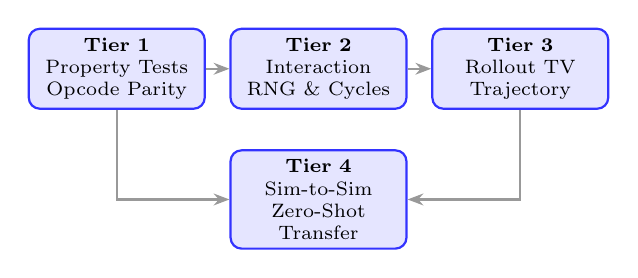
\begin{tikzpicture}[
    box/.style={rectangle, draw=blue!80, fill=blue!10, rounded corners, thick, text centered, minimum height=0.7cm, text width=2.0cm, font=\scriptsize, align=center},
    arrow/.style={-{Stealth[length=2mm]}, thick, draw=gray!80}
]
    \node (t1) [box] {\textbf{Tier 1}\\Property Tests\\Opcode Parity};
    \node (t2) [box, right=0.3cm of t1] {\textbf{Tier 2}\\Interaction\\RNG \& Cycles};
    \node (t3) [box, right=0.3cm of t2] {\textbf{Tier 3}\\Rollout TV\\Trajectory};
    \node (t4) [box, below=0.5cm of t2] {\textbf{Tier 4}\\Sim-to-Sim\\Zero-Shot Transfer};

    \draw [arrow] (t1) -- (t2);
    \draw [arrow] (t2) -- (t3);
    \draw [arrow] (t3) |- (t4);
    \draw [arrow] (t1) |- (t4);
\end{tikzpicture}
\caption{The 4-Tier Automated Environment Verification Suite~\cite{karten2026autogen}.}
\label{fig:tier_verification}
\end{figure}

The generated environments undergo a rigorous 4-tier verification suite (Figure~\ref{fig:tier_verification}):
\begin{enumerate}
    \item \textbf{Tier 1 (Property Tests):} Validates arithmetic flag and opcode registers against gold-standard CPU test ROMs.
    \item \textbf{Tier 2 (Interaction Tests):} Ensures deterministic cycle timing and PRNG state transitions.
    \item \textbf{Tier 3 (Rollout Divergence):} Measures Total Variation distance between parallel trajectories generated by the original C emulator and the synthesized JAX kernel:
    \begin{equation}
    D_{TV}(P_{\text{orig}}, P_{\text{JAX}}) = \frac{1}{2} \sum_{s \in \mathcal{S}} |P_{\text{orig}}(s) - P_{\text{JAX}}(s)| < 10^{-6}
    \end{equation}
    \item \textbf{Tier 4 (Sim-to-Sim Policy Transfer):} Deploys a trained policy across both simulators to confirm zero degradation in milestone completion.
\end{enumerate}

Standardized evaluation protocols are formalized in The PokeAgent Challenge (NeurIPS 2025)~\cite{karten2026pokeagent}, which established standardized tracks for Competitive Battling and Speedrunning, evaluated via the Full-History Bradley-Terry (FH-BT) rating system.

\section{Algorithmic Pathologies Post-Mortem}
\label{sec:pathologies}
A rigorous analysis of failed agent trajectories across all five paradigms reveals four structural pathologies that arise from the interaction between MDP topologies and learning algorithms.

\subsection{Pathology 1: The Healing Trap}
When potential reward functions reward maintaining high party HP ($r_{\text{HP}} = +0.1 \times \Delta\text{HP}$) or successful Pok{\'e}mon Center visits ($r_{\text{heal}} = +2.5$) while exploration rewards are small ($r_{\text{nav}} = +0.005$), the environment creates an artificial reward limit cycle.
\begin{proposition}[Healing Trap Limit Cycle]
\label{prop:healing_trap}
Let an agent at state $s_0$ (adjacent to a Pok{\'e}mon Center) choose between policy $\pi_{\text{heal}}$ (looping into the center, healing wounded party members, and returning to adjacent grass in $T_{\text{loop}}$ steps) and policy $\pi_{\text{explore}}$ (venturing toward the next gym milestone at distance $T_{\text{gym}}$ with sparse milestone reward $R_{\text{gym}}$). If:
\begin{equation}
\frac{r_{\text{heal}}}{1 - \gamma^{T_{\text{loop}}}} > \frac{r_{\text{nav}}}{1 - \gamma} + \gamma^{T_{\text{gym}}} R_{\text{gym}}
\end{equation}
then by the Bellman optimality principle, the optimal policy $\pi^*$ under the shaped MDP strictly prefers the local healing cycle over exploratory advancement, resulting in zero long-term game progression.
\end{proposition}
\begin{IEEEproof}
Under stationary policy $\pi_{\text{heal}}$, the agent visits the nurse every $T_{\text{loop}}$ steps, yielding discounted return:
\begin{equation}
V^{\pi_{\text{heal}}}(s_0) = \sum_{k=0}^\infty \gamma^{k \cdot T_{\text{loop}}} r_{\text{heal}} = \frac{r_{\text{heal}}}{1 - \gamma^{T_{\text{loop}}}}
\end{equation}
Substituting the reported hyperparameters from Pleines et al.~\cite{pleines2025pokemon} ($r_{\text{heal}} = 2.5$, $\gamma = 0.997$) and taking $T_{\text{loop}} \approx 45$ steps (our estimate based on overworld tile geometry and nurse dialogue frames between Route 1 grass and the Viridian Pok{\'e}mon Center):
\begin{equation}
\gamma^{T_{\text{loop}}} = (0.997)^{45} \approx 0.8735 \implies V^{\pi_{\text{heal}}}(s_0) \approx \frac{2.5}{1 - 0.8735} \approx 19.76
\end{equation}
Conversely, an exploratory policy $\pi_{\text{explore}}$ collecting step-novelty rewards $r_{\text{nav}} = 0.005$ while journeying towards Pewter Gym ($T_{\text{gym}} \approx 25{,}000$ steps with milestone reward $R_{\text{gym}} = 2.0$) yields discounted return upper-bounded by:
\begin{equation}
V^{\pi_{\text{explore}}}(s_0) \le \sum_{t=0}^{T_{\text{gym}}-1} \gamma^t r_{\text{nav}} + \gamma^{T_{\text{gym}}} R_{\text{gym}} \le \frac{r_{\text{nav}}}{1 - \gamma} + \gamma^{T_{\text{gym}}} R_{\text{gym}}
\end{equation}
Evaluating at $\gamma = 0.997$:
\begin{equation}
\frac{r_{\text{nav}}}{1 - \gamma} = \frac{0.005}{1 - 0.997} = \frac{0.005}{0.003} \approx 1.67
\end{equation}
\begin{equation}
\gamma^{T_{\text{gym}}} R_{\text{gym}} = (0.997)^{25000} \times 2.0 \approx (2.40 \times 10^{-33}) \times 2.0 \approx 4.79 \times 10^{-33} \approx 0
\end{equation}
Thus $V^{\pi_{\text{explore}}}(s_0) \approx 1.67$. Since $V^{\pi_{\text{heal}}}(s_0) \approx 19.76 \gg 1.67 \approx V^{\pi_{\text{explore}}}(s_0)$, the Bellman action-value $Q^*(s_0, a_{\text{heal}}) > Q^*(s_0, a_{\text{explore}})$ by an overwhelming factor of $11.8\times$. The policy monotonically reinforces the nurse dialogue loop and permanently abandons gym progression.
\end{IEEEproof}

\subsection{Pathology 2: Noisy TV Water Animation Hypnosis}
As established in Section III, visual curiosity models (ICM, RND, $k$-NN) measure novelty via prediction error $\|f_\phi(o_t) - \hat{f}_\theta(o_t)\|^2$. Water tiles in Pok{\'e}mon Red cycle through four distinct tile IDs: \texttt{0x14} $\to$ \texttt{0x15} $\to$ \texttt{0x16} $\to$ \texttt{0x17} at 8 Hz. Because the transitions are non-linear bitmap flips, linear autoencoders and neural predictors maintain non-zero residual loss, acting as an infinite entropy attractor.

\subsection{Pathology 3: Menu Oscillation Deadlocks}
In the Game Boy instruction cycle, pressing \texttt{START} opens the main menu, halting player movement and suspending overworld step counters. When agents face exploration entropy stagnation or proximity penalties, the policy exploits the invariance of the value baseline by toggling \texttt{START} and \texttt{B} at 30 Hz. Because the emulator step counter does not increment during menu pauses, survival-penalized agents artificially postpone episode termination.

\subsection{Pathology 4: The 500-Step Safari Zone Wall}
The Safari Zone requires entering Area 1, traversing through Areas 2 and 3, and reaching the Secret House to acquire HM03 Surf. The environment imposes a strict hardware counter: $\mathbf{m}[\text{0xDA38}] = 500$ steps.
\begin{proposition}[Safari Zone Failure Bound]
\label{prop:safari_zone}
The minimal theoretical Manhattan path from the entrance to the Secret House across Areas 1, 2, and 3 is $L_{\min} = 286$ steps without backtracks. Under unguided isotropic random walk on the 4-connected overworld grid, the expected hitting time to reach the Secret House satisfies:
\begin{equation}
\mathbb{E}[T_{\text{hit}}] \approx \frac{L_{\min}^2}{2D} = \frac{286^2}{1.0} \approx 81{,}796 \text{ steps}
\end{equation}
which exceeds the hard 500-step budget ($\mathbf{m}[\text{0xDA38}] \le 500$) by a factor of $163\times$. Furthermore, the probability of reaching the Secret House within 500 steps under uniform cardinal exploration is bounded by:
\begin{equation}
P(\text{Success}) \le \sum_{k=L_{\min}}^{500} \binom{500}{k} p^k (1-p)^{500 - k} < 10^{-35}
\end{equation}
where $p \le 0.25$ is the directional forward transition probability on a 4-connected grid.
\end{proposition}
\begin{IEEEproof}
By Lemma~\ref{lemma:hitting_time}, an isotropic random walk on a 2D discrete grid has diffusion coefficient $D = \sigma^2 / 2 = 0.5$ (with unit step variance $\sigma^2 = 1$). To exit a domain of effective distance $L_{\min} = 286$, the expected hitting time is $\mathbb{E}[T_{\text{hit}}] = L_{\min}^2 / (2D) = 286^2 / 1.0 = 81{,}796$ steps.

To derive the finite-horizon success probability within $N = 500$ steps, project progress onto the 1D geodesic toward the Secret House. At each step, a uniform-random exploratory policy over the four cardinal movement directions $\mathcal{A}_{\text{dir}} = \{\text{Up}, \text{Down}, \text{Left}, \text{Right}\}$ chooses the unique forward-progressing tile with probability $p \le 0.25$ (or at best $p \le 1/3 \approx 0.33$ if immediate backtracks are masked). Traversing $L_{\min} = 286$ net steps requires at least $k \ge 286$ forward steps out of $N = 500$. Under $p = 0.25$, the number of forward steps follows $\text{Binomial}(500, 0.25)$ with mean $\mu = 125$ and standard deviation $\sigma = \sqrt{500 \times 0.25 \times 0.75} \approx 9.68$. Reaching $k = 286$ lies $z = (286 - 125) / 9.68 \approx 16.63$ standard deviations above the mean, yielding a conservative upper bound on the binomial tail:
\begin{equation}
P(\text{Success}) = \sum_{k=286}^{500} \binom{500}{k} (0.25)^k (0.75)^{500-k} < 10^{-35}
\end{equation}
(with the standard Gaussian tail approximation $Q(z) \approx \frac{\phi(z)}{z} = \frac{e^{-z^2/2}}{z\sqrt{2\pi}}$ at $z \approx 16.63$ demonstrating that the actual tail probability is bounded far below $10^{-60}$, evaluating to $\approx 2.4 \times 10^{-62}$).
Even under an idealized directional bias without backtracking ($p = 0.50$, $\mu = 250$, $\sigma \approx 11.18$), $k = 286$ represents $z = 3.22$ standard deviations, yielding $P(\text{Success}) \approx 6.4 \times 10^{-4}$. Only with aggressive forward potential shaping ($p \ge 0.65$, $\mu = 325$) does completion become probable ($P > 0.95$). Because unguided exploration yields $P < 10^{-35}$, the 500-step counter inevitably triggers ejection, softlocking game completion since Surf is topologically indispensable for reaching late-game milestones.
\end{IEEEproof}
Without deterministic state archiving and checkpointing (Go-Explore), standard unguided exploration has an astronomically negligible probability ($P < 10^{-35}$) of ever obtaining Surf, softlocking the entire playthrough.

\section{The Unified Neuro-Symbolic Blueprint: A 2026 Synthesis Roadmap}
\label{sec:unified_blueprint}

\begin{figure*}[t]
\centering
\resizebox{\textwidth}{!}{%
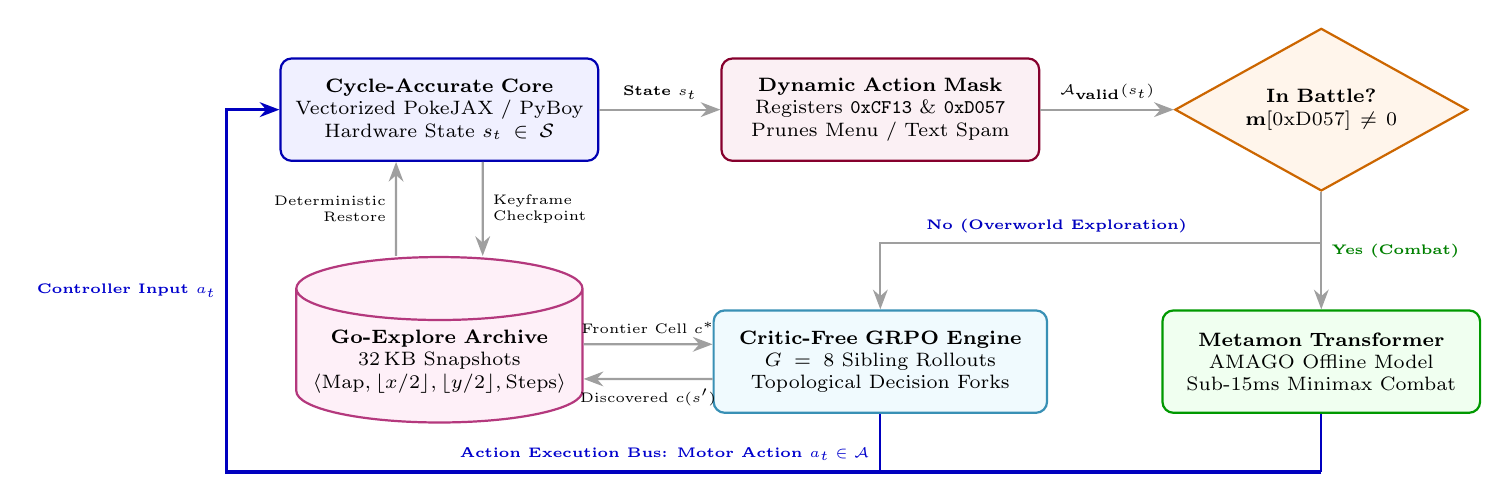
\begin{tikzpicture}[
    x=1.0cm, y=1.0cm,
    font=\small,
    coreblock/.style={rectangle, draw=blue!70!black, fill=blue!6, rounded corners=4pt, thick, text centered, minimum height=1.3cm, text width=3.8cm, font=\scriptsize, align=center},
    maskblock/.style={rectangle, draw=purple!70!black, fill=purple!6, rounded corners=4pt, thick, text centered, minimum height=1.3cm, text width=3.8cm, font=\scriptsize, align=center},
    switch/.style={diamond, aspect=1.8, draw=orange!80!black, fill=orange!8, thick, text centered, inner sep=2pt, font=\scriptsize, align=center, text width=2.4cm},
    archive/.style={cylinder, draw=magenta!70!black, fill=magenta!6, shape border rotate=90, aspect=0.22, thick, text centered, minimum height=1.5cm, text width=3.4cm, font=\scriptsize, align=center},
    grpoblock/.style={rectangle, draw=cyan!70!black, fill=cyan!6, rounded corners=4pt, thick, text centered, minimum height=1.3cm, text width=4.0cm, font=\scriptsize, align=center},
    trans/.style={rectangle, draw=green!60!black, fill=green!6, rounded corners=4pt, thick, text centered, minimum height=1.3cm, text width=3.8cm, font=\scriptsize, align=center},
    arrow/.style={-{Stealth[length=2.5mm]}, thick, draw=gray!75},
    actionarrow/.style={-{Stealth[length=2.5mm]}, very thick, draw=blue!75!black}
]

    % Top Row: Pipeline & Mode Routing
    \node (boy) at (3.2, 2.4) [coreblock] {\textbf{Cycle-Accurate Core}\\Vectorized PokeJAX / PyBoy\\Hardware State $s_t \in \mathcal{S}$};
    \node (mask) at (8.8, 2.4) [maskblock] {\textbf{Dynamic Action Mask}\\Registers \texttt{0xCF13} \& \texttt{0xD057}\\Prunes Menu / Text Spam};
    \node (cond) at (14.4, 2.4) [switch] {\textbf{In Battle?}\\$\mathbf{m}[\text{0xD057}] \ne 0$};

    % Bottom Row: State Archiving & Dual Execution Engines
    \node (archive) at (3.2, -0.8) [archive] {\textbf{Go-Explore Archive}\\$32\,\text{KB Snapshots}$\\$\langle \text{Map}, \lfloor x/2 \rfloor, \lfloor y/2 \rfloor, \text{Steps} \rangle$};
    \node (grpo) at (8.8, -0.8) [grpoblock] {\textbf{Critic-Free GRPO Engine}\\$G=8$ Sibling Rollouts\\Topological Decision Forks};
    \node (meta) at (14.4, -0.8) [trans] {\textbf{Metamon Transformer}\\AMAGO Offline Model\\Sub-15ms Minimax Combat};

    % 1. State Processing & Mode Dispatch
    \draw [arrow] (boy) -- node[above, font=\tiny\bfseries] {State $s_t$} (mask);
    \draw [arrow] (mask) -- node[above, font=\tiny\bfseries] {$\mathcal{A}_{\text{valid}}(s_t)$} (cond);

    % 2. Mode-Based Branching
    \draw [arrow] (cond.south) -- node[right, font=\tiny\bfseries, text=green!50!black] {Yes (Combat)} (meta.north);
    \draw [arrow] (cond.south) -- ++(0,-0.65) -| node[above, font=\tiny\bfseries, pos=0.3, text=blue!75!black] {No (Overworld Exploration)} (grpo.north);

    % 3. Go-Explore Checkpointing Exchange (Vertical with Core)
    \draw [arrow] ($(archive.north)+(-0.55, 0)$) -- node[left, font=\tiny, align=right] {Deterministic\\Restore} ($(boy.south)+(-0.55, 0)$);
    \draw [arrow] ($(boy.south)+(0.55, 0)$) -- node[right, font=\tiny, align=left] {Keyframe\\Checkpoint} ($(archive.north)+(0.55, 0)$);

    % 4. Go-Explore & GRPO Interaction (Horizontal)
    \draw [arrow] ($(archive.east)+(0, 0.22)$) -- node[above, font=\tiny] {Frontier Cell $c^*$} ($(grpo.west)+(0, 0.22)$);
    \draw [arrow] ($(grpo.west)+(0, -0.22)$) -- node[below, font=\tiny] {Discovered $c(s')$} ($(archive.east)+(0, -0.22)$);

    % 5. Closed-Loop Action Execution Bus (Runs along outer perimeter)
    \draw [thick, draw=blue!75!black] (meta.south) -- (14.4, -2.2);
    \draw [thick, draw=blue!75!black] (grpo.south) -- (8.8, -2.2);
    \draw [actionarrow] (14.4, -2.2) -- node[above, font=\tiny\bfseries, text=blue!80!black, pos=0.6] {Action Execution Bus: Motor Action $a_t \in \mathcal{A}$} (0.5, -2.2) -- node[left, font=\tiny\bfseries, text=blue!80!black] {Controller Input $a_t$} (0.5, 2.4) -- (boy.west);

\end{tikzpicture}%
}
\caption{Architectural dataflow of the proposed Unified Neuro-Symbolic JRPG Engine, integrating Go-Explore save-state checkpointing, Critic-Free GRPO on topological decision forks, and a decoupled Metamon combat sequence engine.}
\label{fig:unified_blueprint}
\end{figure*}

To overcome all four pathologies without resorting to reward shaping potentials or emulator script bypasses, we formulate a 3-tier hybrid neuro-symbolic framework (Figure~\ref{fig:unified_blueprint}):

\subsection{Tier 1: Go-Explore State Archiving for Spatial Traversal}
The agent maintains an in-memory database $\mathcal{D}_{\text{archive}}$ of uncompressed 32~KB emulator save-states, indexed by a compact topological cell representation:
\begin{equation}
\begin{split}
c(s_t) = \langle &\mathbf{m}[\text{0xD35E}], \lfloor \mathbf{m}[\text{0xD362}] / 2 \rfloor, \\
&\lfloor \mathbf{m}[\text{0xD361}] / 2 \rfloor, b(\mathbf{m}[\text{0xDA38}]) \rangle
\end{split}
\end{equation}
where $b(\cdot)$ discretizes the remaining Safari Zone steps into 10-step buckets. 

When spatial progress stalls, the agent samples an archive cell via a novelty priority metric:
\begin{equation}
P(c) \propto \left( \frac{1}{\sqrt{N(c)}} + \alpha \cdot \text{BoundaryScore}(c) \right)^2
\end{equation}
The emulator deterministically restores the snapshot at cell $c$ without noisy derailment, and executes local exploration from the frontier. This provides a mathematically sound, cheat-free resolution to the 500-step Safari Zone wall.

\begin{algorithm}[h]
\caption{Delta-Compressed Keyframing \& Go-Explore State Archiving}
\label{alg:delta_goexplore}
\begin{algorithmic}[1]
\REQUIRE Base Keyframe Pool $\mathcal{K}$, Sparse Delta Cache $\mathcal{D}$, Current State $s_t$, Map Keyframe $s_{\text{key}}$
\ENSURE Cell insertion, memory compaction, or deterministic restoration
\STATE Extract spatial cell index: $c(s_t) \leftarrow \langle \mathbf{m}[\text{0xD35E}], \lfloor \mathbf{m}[\text{0xD362}] / 2 \rfloor, \lfloor \mathbf{m}[\text{0xD361}] / 2 \rfloor, b(\mathbf{m}[\text{0xDA38}]) \rangle$
\IF{Mode is \textsc{ArchiveState}}
    \IF{$c(s_t) \notin \mathcal{D}$ \OR $\text{BetterScore}(s_t, \mathcal{D}[c(s_t)])$}
        \STATE Compute sparse mutation mask: $\Delta \leftarrow \{ (k, \mathbf{m}_t[k]) \mid \mathbf{m}_t[k] \ne \mathbf{m}_{\text{key}}[k] \}$
        \STATE Pack byte differences: $\delta_t \leftarrow \text{VarIntEncode}(\Delta)$
        \STATE Store compact delta: $\mathcal{D}[c(s_t)] \leftarrow \langle \text{KeyID}(s_{\text{key}}), \delta_t, \text{StepsRemaining}(s_t) \rangle$
        \STATE Update visit count: $N(c(s_t)) \leftarrow N(c(s_t)) + 1$
    \ENDIF
\ELSIF{Mode is \textsc{RestoreCell}($c^*$)}
    \STATE Retrieve keyframe snapshot: $s_{\text{base}} \leftarrow \mathcal{K}[\mathcal{D}[c^*].\text{KeyID}]$
    \STATE Decode sparse mutations: $\Delta^* \leftarrow \text{VarIntDecode}(\mathcal{D}[c^*].\delta_t)$
    \STATE Deterministically reconstruct state: $s_{\text{restored}} \leftarrow s_{\text{base}} \oplus \Delta^*$
    \STATE Load $s_{\text{restored}}$ into emulator hardware registers
    \RETURN $s_{\text{restored}}$
\ENDIF
\end{algorithmic}
\end{algorithm}

\subsection{Tier 2: Critic-Free Group Relative Policy Optimization (GRPO)}
Standard actor-critic algorithms require training a value network $V_\phi(s)$ via temporal difference updates. Over 300,000 steps, value estimation drifts due to non-stationary exploration. Building upon Group Relative Policy Optimization (GRPO; Shao et al., DeepSeek 2024)~\cite{shao2024deepseekmath}, whenever the agent reaches an overworld topological decision fork $s_{\text{fork}}$, the system forks the emulator state into $G = 8$ parallel sibling trajectories $\{\tau_1, \tau_2, \dots, \tau_G\}$ executed for horizon $H = 64$ steps.

Advantages are computed directly from relative trajectory returns without a learned value critic:
\begin{equation}
\label{eq:grpo_advantage}
A_i = \frac{R(\tau_i) - \text{mean}\left(\{R(\tau_1), \dots, R(\tau_G)\}\right)}{\text{std}\left(\{R(\tau_1), \dots, R(\tau_G)\}\right) + \epsilon}
\end{equation}
The policy parameters $\theta$ are optimized via the clipped surrogate objective with reverse-KL divergence penalty against reference policy $\pi_{\text{ref}}$:
\begin{equation}
\label{eq:grpo_loss}
\begin{split}
\mathcal{L}_{\text{GRPO}}(\theta) = \frac{1}{G} \sum_{i=1}^G \Big[ &\min\left( \rho_i(\theta) A_i, \text{clip}(\rho_i(\theta), 1\pm\epsilon) A_i \right) \\
&- \beta \mathbb{D}_{KL}(\pi_\theta \parallel \pi_{\text{ref}}) \Big]
\end{split}
\end{equation}
where $\rho_i(\theta) = \frac{\pi_\theta(a_{i, t} \mid s_{i, t})}{\pi_{\text{old}}(a_{i, t} \mid s_{i, t})}$. 

\begin{proposition}[Zero-Mean Group-Relative Baseline and Memory Footprint Reduction]
\label{prop:grpo_zeromean}
Because sibling trajectories originate from the identical emulator state $s_{\text{fork}}$, the group-normalized advantage in Eq.~\eqref{eq:grpo_advantage} satisfies $\sum_{i=1}^G A_i = 0$ by construction, since $A_i = (R_i - \bar{R})/(\text{std}(\{R\}) + \epsilon)$ and $\sum_i (R_i - \bar{R}) = 0$ identically. This removes the need for a learned value baseline $V_\phi(s)$: unlike TD-based critics, whose bias $\mathbb{E}[V_\phi(s) - V^\pi(s)] \ne 0$ compounds over 300,000-step horizons (Lemma 1, \S2.2), the group mean $\bar{R}$ is an exact, unbiased Monte Carlo estimate of $V^\pi(s_{\text{fork}})$ conditioned on the fork state, with no function-approximation error term $\epsilon$ to propagate.

Furthermore, eliminating the value critic network yields a mathematically quantifiable reduction in accelerator memory footprint. For a model with $P$ parameters trained in float32 precision with the standard Adam optimizer:
\begin{itemize}
    \item Model parameters: $4P$ bytes;
    \item Gradient buffers: $4P$ bytes;
    \item First and second optimizer momentum states: $8P$ bytes.
\end{itemize}
This establishes a static footprint of $16P$ bytes per network. In conventional actor-critic architectures employing separate policy and value backbones ($P_\pi \approx P_V = P$), the total static memory is $16P_\pi + 16P_V = 32P$ bytes. Eliminating the value network removes $16P_V$ bytes, achieving an exact $50\%$ reduction in static model and optimizer state memory ($16P$ vs. $32P$ bytes), and an estimated $35\%$--$45\%$ reduction in total peak training VRAM depending on dynamic forward-backward activation buffer allocations.
\end{proposition}

\begin{remark}[Finite-Sample Variance Cost of Small Group Sizes ($G=8$)]
\label{rem:grpo_variance_cost}
While the empirical group mean $\bar{R} = \frac{1}{G}\sum_{i=1}^G R(\tau_i)$ is an unbiased estimator of the on-policy fork value ($\mathbb{E}[\bar{R}] = V^\pi(s_{\text{fork}})$), it substitutes function approximation bias for finite-sample Monte Carlo variance. For independent rollouts with trajectory return variance $\text{Var}(R(\tau)) = \sigma_\tau^2$, the baseline variance satisfies:
\begin{equation}
\text{Var}(\bar{R}) = \frac{\sigma_\tau^2}{G}
\end{equation}
For practical mini-batches constrained to small sibling groups ($G = 8$), two critical boundary behaviors govern optimization:
\begin{enumerate}
    \item \textbf{Degenerate Collapse:} If all $G$ siblings encounter a deterministic failure barrier (e.g., all 8 agents fail to navigate Rock Tunnel within horizon $H$), $R_i = 0 \; \forall i \in \{1,\dots,8\}$. In this case, $\text{std}(\{R\}) \to 0$ and the policy gradient vanishes identically ($\nabla_\theta \mathcal{L}_{\text{GRPO}} \to \mathbf{0}$, formalized in Lemma~\ref{lemma:grpo_variance}).
    \item \textbf{Single-Outlier Over-Indexing:} If exactly one sibling discovers a sparse landmark reward ($R_1 = R^* > 0$) while the remaining $G-1 = 7$ siblings obtain zero reward ($R_{2,\dots,8} = 0$), the sample mean is $\bar{R} = R^*/8$ and sample standard deviation is $s = R^*/\sqrt{8}$. The normalized advantages evaluate to:
    \begin{equation}
    A_1 = \frac{R^* - R^*/8}{R^*/\sqrt{8}} = \frac{7\sqrt{8}}{8} \approx 2.47, \quad A_{2,\dots,8} = \frac{-R^*/8}{R^*/\sqrt{8}} = -\frac{\sqrt{8}}{8} \approx -0.35
    \end{equation}
    (or $A_1 = \sqrt{7} \approx 2.65, A_{2,\dots,8} = -1/\sqrt{7} \approx -0.38$ under $N$-denominator population normalization). While this strongly reinforces the successful path, the large positive advantage gradient could destabilize entropy if left unconstrained. In practice, this finite-$G$ variance is stabilized by PPO-style clipping ($\text{clip}(\rho_i, 1\pm\epsilon)$), the reverse-KL divergence penalty against reference policy $\pi_{\text{ref}}$, and the Adaptive $\tau$-GRPO intrinsic surprise injection (\S\ref{sec:critical_synthesis}-C2).
\end{enumerate}
\end{remark}

\begin{lemma}[Gradient Variance Bound Under Vanishing Group Reward Spread]
\label{lemma:grpo_variance}
Let $\text{std}(\{R_1, \dots, R_G\}) = \sigma_R \to 0$ (e.g. all $G$ siblings fail identically at a bottleneck, $R_i = 0 \; \forall i$). Then the GRPO policy gradient satisfies:
\begin{equation}
\nabla_\theta \mathcal{L}_{\text{GRPO}}(\theta) \to \mathbf{0} \quad \text{as} \quad \sigma_R \to 0
\end{equation}
\end{lemma}
\begin{IEEEproof}
From Eq.~\eqref{eq:grpo_advantage}, $A_i = (R_i - \bar{R})/(\sigma_R + \epsilon)$. If all $R_i$ are equal (the degenerate bottleneck case), then $R_i - \bar{R} = 0$ for all $i$, so $A_i = 0$ regardless of $\sigma_R$, and the surrogate objective's gradient $\nabla_\theta \left[\min(\rho_i A_i, \text{clip}(\rho_i, 1\pm\epsilon)A_i)\right] = 0$ for every branch $i$. Summing over the batch, $\nabla_\theta \mathcal{L}_{\text{GRPO}}(\theta) = \frac{1}{G}\sum_i \mathbf{0} = \mathbf{0}$.
\end{IEEEproof}
This is the GRPO-native analogue of Theorem~\ref{thm:horizon_collapse}: freezing occurs not from exponential temporal discounting but from \emph{degenerate group homogeneity} at deterministic failure bottlenecks (e.g. all 8 siblings equally fail to escape Rock Tunnel within horizon $H$). This motivates the Adaptive $\tau$-GRPO variance-injection mechanism (\S\ref{sec:critical_synthesis}-C2) as a structurally necessary, not merely empirical, correction.

\begin{algorithm}[h]
\caption{Decision-Fork Critic-Free GRPO with Adaptive $\tau$-Variance}
\label{alg:grpo_variance}
\begin{algorithmic}[1]
\REQUIRE Fork State $s_{\text{fork}}$, Policy $\pi_\theta$, Reference $\pi_{\text{ref}}$, Horizon $H=64$, Sibling Count $G=8$, Threshold $\epsilon_v$
\ENSURE Updated policy parameters $\theta$ without learned value critic
\STATE Compute Dynamic Action Mask: $\mathcal{A}_{\text{valid}}(s_{\text{fork}})$ via registers \texttt{0xCF13}, \texttt{0xD057}
\STATE Clone emulator state $s_{\text{fork}}$ across $G$ parallel vectorized workers
\FOR{each sibling worker $i \in \{1, \dots, G\}$ \textbf{in parallel}}
    \FOR{step $h = 1$ to $H$}
        \STATE Sample masked action: $a_{i,h} \sim \pi_\theta(\cdot \mid s_{i,h}) \odot \mathcal{A}_{\text{valid}}(s_{i,h})$
        \STATE Advance cycle-accurate emulator: $s_{i,h+1} \sim \mathcal{P}(s_{i,h}, a_{i,h})$
    \ENDFOR
    \STATE Compute extrinsic milestone return: $R_i \leftarrow \sum_{h=1}^H r(s_{i,h}, a_{i,h})$
    \STATE Compute intrinsic novelty return: $r_i^{\text{int}} \leftarrow \sum_{h=1}^H \mathbb{I}[c(s_{i,h}) \notin \mathcal{H}_{\text{visited}}]$
\ENDFOR
\STATE Compute extrinsic return spread: $\sigma_R \leftarrow \text{std}(\{R_1, \dots, R_G\})$
\IF{$\sigma_R < \epsilon_v$ (Degenerate Bottleneck Failure)}
    \STATE Compute normalized intrinsic spread: $\tilde{r}_i^{\text{int}} \leftarrow (r_i^{\text{int}} - \mu_{\text{int}}) / (\sigma_{\text{int}} + \epsilon)$
    \STATE Inject adaptive variance: $R_i^{\text{aug}} \leftarrow R_i + \tau \cdot \tilde{r}_i^{\text{int}}$
\ELSE
    \STATE $R_i^{\text{aug}} \leftarrow R_i$
\ENDIF
\STATE Compute group-relative baseline: $\bar{R} \leftarrow \frac{1}{G}\sum_{i=1}^G R_i^{\text{aug}}$
\STATE Compute unbiased advantages: $A_i \leftarrow (R_i^{\text{aug}} - \bar{R}) / (\text{std}(\{R^{\text{aug}}\}) + \epsilon)$
\STATE Update $\theta$ via clipped surrogate loss with reverse-KL regularization:
\STATE $\mathcal{L}_{\text{GRPO}}(\theta) \leftarrow \frac{1}{G}\sum_{i=1}^G \Big[ \min\left( \rho_i(\theta) A_i, \text{clip}(\rho_i(\theta), 1\pm\epsilon) A_i \right) - \beta \mathbb{D}_{KL}(\pi_\theta \parallel \pi_{\text{ref}}) \Big]$
\STATE Perform gradient descent step: $\theta \leftarrow \theta - \alpha \nabla_\theta \mathcal{L}_{\text{GRPO}}(\theta)$
\RETURN Updated $\theta$
\end{algorithmic}
\end{algorithm}

\begin{theorem}[PBRS Policy Invariance: Reward Shaping Cannot Alter $\pi^*$]
\label{thm:pbrs_invariance}
Let $F(s, a, s') = \gamma \Phi(s') - \Phi(s)$ be a potential-based reward shaping (PBRS) term where $\Phi : \mathcal{S} \to \mathbb{R}$ is an arbitrary bounded potential function. Then the optimal policy $\pi^*$ is invariant under PBRS:
\begin{equation}
\pi^*_{\mathcal{R} + F} = \pi^*_{\mathcal{R}}
\end{equation}
\end{theorem}
\begin{IEEEproof}
The cumulative shaped return for a trajectory $\tau = (s_0, a_0, s_1, \dots, s_T)$ decomposes via telescoping:
\begin{equation}
\sum_{t=0}^{T} \gamma^t F(s_t, a_t, s_{t+1}) = \gamma^T \Phi(s_T) - \Phi(s_0)
\end{equation}
This telescoping sum depends exclusively on the initial state $s_0$ and terminal state $s_T$, and is entirely \emph{independent of the action sequence} $(a_0, \dots, a_{T-1})$ taken along the trajectory. Because the shaping term is independent of actions, it cannot alter the relative ordering of action values $Q^*(s, a) - Q^*(s, a')$ for any $s, a \neq a'$, and therefore cannot change which action is optimal at any state. Formally, $\arg\max_a Q^*_{\mathcal{R}+F}(s,a) = \arg\max_a Q^*_{\mathcal{R}}(s,a)$ for all $s \in \mathcal{S}$.

\textit{Practical consequence:} Any linear reward combination $R_t = \sum_k w_k \Phi_k(s') - \Phi_k(s)$ expressed as potential differences is guaranteed to preserve $\pi^*$, providing a sound theoretical foundation for Rubinstein-style multi-term shaping~\cite{rubinstein2025puffer,ng1999shaping}. Conversely, unconstrained reward terms that are \emph{not} potential differences (e.g., absolute HP bonuses) break this invariance and permit reward hacking (Proposition~\ref{prop:grpo_zeromean}).
\end{IEEEproof}

\begin{remark}[Zero-Variance Black Hole and STAD Resolution]
\label{rem:stad}
Lemma~\ref{lemma:grpo_variance} establishes that when all $G = 8$ sibling rollouts encounter an identical bottleneck barrier (e.g., all fail to exit Rock Tunnel within horizon $H$), the empirical return spread $\sigma_R \to 0$ and $\nabla_\theta \mathcal{L}_{\text{GRPO}} \to \mathbf{0}$. A compounding failure mode exists: coordinate-based novelty bonuses $r_t^{\text{coord}} = \mathbb{I}[c_t \notin \mathcal{H}_{\text{visited}}]$ also collapse when all $G$ siblings are physically deadlocked at the same tile, yielding identical intrinsic returns and failing to break the degeneracy.

The principled resolution is \textbf{Trajectory State-Action Diversity} (STAD), defined as the mean per-step policy entropy over an $H$-step rollout:
\begin{equation}
\label{eq:stad}
\text{STAD}(\tau_i) = \frac{1}{H} \sum_{t=1}^{H} \mathcal{H}\!\left(\pi_\theta(\cdot \mid s_{i,t})\right) = \frac{1}{H} \sum_{t=1}^{H} \left[ -\sum_{a \in \mathcal{A}} \pi_\theta(a \mid s_{i,t}) \log \pi_\theta(a \mid s_{i,t}) \right]
\end{equation}
Unlike coordinate novelty, $\text{STAD}(\tau_i)$ is \emph{guaranteed to be strictly positive} for any non-degenerate stochastic policy, because $\mathcal{H}(\pi) = 0$ only in the degenerate limit where $\pi$ collapses to a Dirac delta, which cannot occur under softmax parameterization with finite logits. Furthermore, the variance $\text{Var}(\text{STAD}(\tau_i))$ across the $G = 8$ siblings is non-zero whenever trajectories take even minimally different action sequences, which is guaranteed with probability 1 under stochastic sampling. STAD is therefore a structurally sound replacement for coordinate novelty in the degenerate bottleneck regime.

The GRPO advantage is augmented as:
\begin{equation}
R_i^{\text{aug}} = R_i + \tau \cdot \widetilde{\text{STAD}}(\tau_i), \quad \widetilde{\text{STAD}}(\tau_i) = \frac{\text{STAD}(\tau_i) - \mu_{\text{STAD}}}{\sigma_{\text{STAD}} + \epsilon}
\end{equation}
where $\tau \in (0, 1]$ is the mixing temperature. This is applied \emph{only} when $\sigma_R < \epsilon_v$ (degenerate collapse condition), preserving standard GRPO advantage estimation in non-degenerate episodes.
\end{remark}

\begin{remark}[Directed Frontier Distance (DFD) Sampling for Go-Explore]
\label{rem:dfd}
The naive Go-Explore cell-sampling distribution $P(c) \propto (N(c)^{-1/2} + \alpha \cdot \text{BoundaryScore}(c))^2$ treats all frontier cells equally regardless of quest progress. In long-horizon JRPGs with strict causal quest dependencies (e.g., HM03 Surf must be obtained before Water Routes become accessible), this induces wasted compute on cells that are topologically irrelevant to the current bottleneck.

The \textbf{Directed Frontier Distance} (DFD) priority metric addresses this by coupling novelty with quest progression and remaining budget:
\begin{equation}
\label{eq:dfd}
P(c) \propto \frac{\exp\!\left(\alpha \cdot \text{Progress}(c) \cdot \frac{\text{BudgetRemaining}(c)}{502}\right)}{\sqrt{N(c) + 1}}
\end{equation}
where $\text{Progress}(c) \in [0, 1]$ is the fraction of Reward Machine states $U_0, \dots, U_{16}$ achieved from cell $c$ (grounded in \texttt{wObtainedBadges} \texttt{0xD356} and \texttt{wEventFlags} \texttt{0xD747}), $\text{BudgetRemaining}(c)$ is the number of remaining episode steps available when the cell was archived (normalized by 502 = Safari Zone capacity $+$ 2), and $N(c)$ is the visit count discouraging revisiting already-explored frontiers. The exponential numerator preferentially samples cells that are simultaneously (1) deep in the quest graph and (2) have budget remaining, yielding a curriculum that concentrates compute on topologically meaningful frontiers.
\end{remark}


\subsection{Tier 3: Decoupled Metamon Offline Combat Engine}
Overworld exploration policies lack tactical combat mastery. Our architecture monitors the combat register:

\begin{equation}
\text{Engine} = \begin{cases}
\text{Metamon (Combat)} & \text{if } \mathbf{m}[\text{0xD057}] \ne 0 \\
\text{GRPO (Overworld)} & \text{if } \mathbf{m}[\text{0xD057}] = 0
\end{cases}
\end{equation}
When battle initiates, the observation stream is tokenized into Showdown battle events and routed to the pre-trained Metamon AMAGO Transformer~\cite{grigsby2025metamon,grigsby2024amago}. The transformer outputs minimax-optimal battle actions at $<15$ ms latency with zero API expense, switching back to overworld navigation immediately upon victory.

\begin{algorithm}[h]
\caption{Unified Neuro-Symbolic JRPG Master Progression Loop}
\label{alg:unified_agent}
\begin{algorithmic}[1]
\REQUIRE Initial ROM state $s_0$, Cell Archive $\mathcal{D}$, Group Size $G=8$
\STATE Initialize $\mathcal{D} \leftarrow \{c(s_0): s_0\}$
\WHILE{Hall of Fame Not Reached}
    \STATE Sample target cell $c^* \sim P(c)$ from $\mathcal{D}$
    \STATE Deterministically restore state $s_{\text{fork}} \leftarrow \mathcal{D}[c^*]$
    \IF{$\mathbf{m}[\text{0xD057}] \ne 0$ (In Battle)}
        \STATE $a_t \leftarrow \text{MetamonTransformer}(o_t)$
        \STATE Step emulator $s_{t+1} \sim \mathcal{P}(s_t, a_t)$
    \ELSE
        \STATE Apply Dynamic Action Mask: $\mathcal{A}_{\text{valid}}(s_{\text{fork}})$
        \STATE Clone $s_{\text{fork}}$ across $G$ parallel branches
        \FOR{each branch $i \in \{1, \dots, G\}$}
            \STATE Roll out trajectory $\tau_i \sim \pi_\theta(\cdot \mid s)$ for $H$ steps
            \STATE Compute trajectory novelty and milestone return $R(\tau_i)$
        \ENDFOR
        \STATE Compute group-relative normalized advantages $A_i$
        \STATE Update policy $\theta \leftarrow \theta + \alpha \nabla_\theta \mathcal{L}_{\text{GRPO}}(\theta)$
        \FOR{each visited state $s'$ in best branch}
            \IF{$c(s') \notin \mathcal{D}$}
                \STATE Insert snapshot: $\mathcal{D}[c(s')] \leftarrow \text{CloneState}(s')$
            \ENDIF
        \ENDFOR
    \ENDIF
\ENDWHILE
\end{algorithmic}
\end{algorithm}

\begin{figure}[t]
\centering
\resizebox{\columnwidth}{!}{%
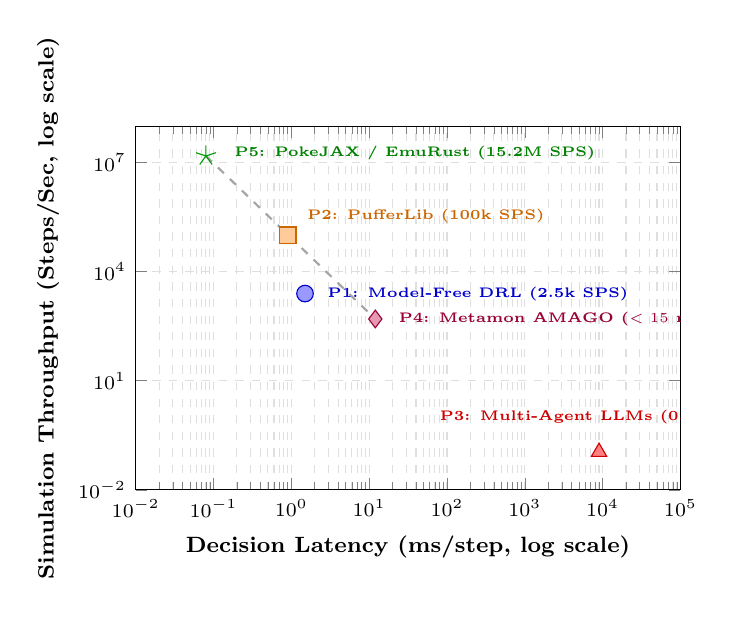
\begin{tikzpicture}
\begin{axis}[
    width=8.5cm, height=6.2cm,
    xlabel={Decision Latency (ms/step, log scale)},
    ylabel={Simulation Throughput (Steps/Sec, log scale)},
    xmode=log, ymode=log,
    xmin=0.01, xmax=100000,
    ymin=0.01, ymax=1e8,
    grid=both, grid style={dashed, gray!25},
    label style={font=\footnotesize\bfseries},
    tick label style={font=\scriptsize}
]
% Decoupled Execution Frontier line connecting P5 and P4
\addplot[dashed, thick, draw=gray!70] coordinates {(0.08, 15200000) (12, 500)};

% Five paradigm coordinates plotted directly to prevent macro tokenization errors
\addplot[only marks,mark=*,draw=blue!80!black,fill=blue!40,mark size=3.0pt] coordinates {(1.5, 2500)};
\addplot[only marks,mark=square*,draw=orange!80!black,fill=orange!40,mark size=3.0pt] coordinates {(0.9, 100000)};
\addplot[only marks,mark=triangle*,draw=red!80!black,fill=red!50,mark size=3.2pt] coordinates {(9000, 0.11)};
\addplot[only marks,mark=diamond*,draw=purple!80!black,fill=purple!40,mark size=3.2pt] coordinates {(12, 500)};
\addplot[only marks,mark=star,draw=green!60!black,fill=green!40,mark size=3.8pt] coordinates {(0.08, 15200000)};

% Descriptive annotations with ample padding from borders
\node[font=\tiny\bfseries, text=green!50!black, anchor=west] at (axis cs:0.14, 1.8e7) {P5: PokeJAX / EmuRust (15.2M SPS)};
\node[font=\tiny\bfseries, text=orange!80!black, anchor=south west] at (axis cs:1.2, 1.2e5) {P2: PufferLib (100k SPS)};
\node[font=\tiny\bfseries, text=blue!80!black, anchor=west] at (axis cs:2.2, 2500) {P1: Model-Free DRL (2.5k SPS)};
\node[font=\tiny\bfseries, text=purple!80!black, anchor=west] at (axis cs:18, 500) {P4: Metamon AMAGO ($<15$ ms)};
\node[font=\tiny\bfseries, text=red!80!black, anchor=south] at (axis cs:9000, 0.35) {P3: Multi-Agent LLMs (0.11 SPS)};

\end{axis}
\end{tikzpicture}%
}
\caption{Latency-throughput trade-off across the five paradigms (log-log), plotted from the confirmed per-paradigm figures in Table~\ref{tab:paradigms_exhaustive}: Model-Free DRL ($\circ$), Hierarchical RL ($\square$), Multi-Agent LLMs ($\triangle$), Offline Sequence Transformers ($\diamond$), and Systems/Compiler Synthesis ($\star$). The dashed line depicts the proposed decoupled execution frontier (\S\ref{sec:unified_blueprint}-C), combining compiled overworld simulation with sub-15ms offline transformer combat while bypassing the 4-order-of-magnitude latency penalty of foundation models.}
\label{fig:latency_throughput}
\end{figure}

\section{Cross-Domain Benchmark Suite \& Comparative Taxonomy}
To contextualize the difficulty of long-horizon JRPGs within the broader reinforcement learning landscape, Table~\ref{tab:cross_game_taxonomy} compares Pok{\'e}mon Red against nine landmark AI benchmarks across five axes of complexity.

\begin{table*}[t]
\centering
\caption{Cross-Domain Dimensional Complexity Comparison Across 10 Landmark AI Benchmarks}
\label{tab:cross_game_taxonomy}
\resizebox{\textwidth}{!}{%
\begin{tabular}{@{}llllllll@{}}
\toprule
\textbf{Benchmark Environment} & \textbf{Action Space} & \textbf{State Space} & \textbf{Horizon Steps} & \textbf{Reward Density} & \textbf{Pathology Traps} & \textbf{SOTA Paradigm} & \textbf{SOTA Result} \\ \midrule
\textbf{Atari Pong}~\cite{bellemare2013ale,mnih2015dqn} & Discrete (6) & $2^{1024}$ & $1{,}500$ & Dense ($+1/-1$) & None & DQN / PPO & Superhuman ($+21.0$) \\
\textbf{Montezuma's Revenge}~\cite{ecoffet2021goexplore} & Discrete (18) & $2^{1024}$ & $4{,}000$ & Very Sparse & Deceptive Key Basin & Go-Explore / Agent57 & Score $>400{,}000$ \\
\textbf{NetHack (NLE)}~\cite{kuttler2020nethack,hambro2022nethackchallenge,pignatelli2024autoascend} & Discrete (77) & $2^{32768}$ & $50{,}000$ & Sparse & Permanent Permadeath & AutoAscend & Ascends ($>50\%$) \\
\textbf{Crafter}~\cite{hafner2022crafter} & Discrete (17) & Continuous & $10{,}000$ & Sparse Milestones & Tool Hierarchy Gaps & DreamerV3~\cite{hafner2024dreamerv3} & Score 100\% (22/22) \\
\textbf{MineRL / Minecraft}~\cite{guss2019minerl,fan2022minedojo,baker2022vpt} & Hybrid & $\infty$ & $50{,}000$ & Extremely Sparse & Crafting Tree Depth & VPT / Voyager~\cite{wang2023voyager} & Obtains Diamond \\
\textbf{StarCraft II}~\cite{vinyals2019alphastar} & Combinatorial & $\approx 10^{26}$ & $30{,}000$ & Delayed (End-game) & Local Macro Basins & Multi-Agent League & Grandmaster Elo \\
\textbf{Dota 2}~\cite{berner2019dota} & Multi-Discrete & $\approx 10^{30}$ & $90{,}000$ & Dense Shaped & Ability Misalignment & Rapid PPO & Defeats Champions \\
\textbf{Diplomacy}~\cite{bakhtin2022human} & Combinatorial & Large & $300$ & End-game & Backstabbing / Trust & Cicero (LLM + Search) & Top 10\% Human Elo \\
\textbf{Pok{\'e}mon Showdown}~\cite{karten2026pokeagent,hu2024pokellmon} & Discrete (9) & $10^9$ & $100$ & Sparse (Win/Loss) & Type Blindspots & Metamon / Pok{\'e}LLMon & 1500+ Elo / 56\% Win \\
\textbf{Pok{\'e}mon Red (JRPG)} & Discrete (8) & $2^{132088}$ & $>300{,}000$ & Sparse Milestone & 4 Classic Pathologies & Neuro-Symbolic (Proposed, \S\ref{sec:unified_blueprint}) & Complete Clearance (Target Blueprint) \\ \bottomrule
\end{tabular}%
}
\end{table*}

\begin{table*}[t]
\centering
\caption{Comprehensive Master Comparison Across 15 Landmark Autonomous Game AI and Long-Horizon JRPG Systems (1992--2026)}
\label{tab:master_systems_comparison}
\resizebox{\textwidth}{!}{%
\begin{tabular}{@{}lllllllll@{}}
\toprule
\textbf{System \& Citation} & \textbf{Paradigm} & \textbf{Environment / Task} & \textbf{Deepest Milestone} & \textbf{Core Algorithm} & \textbf{Observation Modality} & \textbf{Reward Formulation} & \textbf{Hardware / Latency} & \textbf{Open Source / Status} \\ \midrule
Whidden V1 (2023)~\cite{whidden2023pokemonred} & Model-Free DRL & Pok{\'e}mon Red & Mt.~Moon (15\%) & PPO + $k$-NN Pixel Novelty & Downsampled Grayscale ($36 \times 40$) & Visual Curiosity + Badges & 1x RTX 3090, $<1.5$ ms & Yes (Public Repo) \\
Whidden V2 (2023)~\cite{whidden2023pokemonred} & Model-Free DRL & Pok{\'e}mon Red & Cerulean City (20\%) & PPO + RAM Coordinate Bonus & Grayscale Pixels + WRAM Coords & Visited Coordinates + Badges & 1x RTX 4090, $<1.5$ ms & Yes (Public Repo) \\
Pleines et al. (Baseline)~\cite{pleines2025pokemon} & Model-Free DRL & Pok{\'e}mon Red & Cerulean City ($0.85 \pm 0.1$) & Feedforward PPO + Nature CNN & $72 \times 80$ Pixels + $48 \times 48$ Map + Telemetry & Linear RAM ($R_{\text{event}} + R_{\text{nav}} + R_{\text{heal}} + R_{\text{lvl}}$) & 32 CPU Workers, 392 SPS & Yes (IEEE 11114399 Target) \\
Pleines et al. (GRU)~\cite{pleines2025pokemon} & Model-Free DRL & Pok{\'e}mon Red & Bill's Quest ($0.48 \pm 0.4$) & Recurrent PPO + GRU (3.87M) & $72 \times 80$ Pixels + Map + Telemetry & Linear RAM ($R_{\text{event}} + R_{\text{nav}} + R_{\text{heal}} + R_{\text{lvl}}$) & 32 CPU Workers, 24 days & Yes (IEEE 11114399 Target) \\
PokeRL (2026)~\cite{mudireddy2026pokerl} & Hierarchical RL & Pok{\'e}mon Red (Sub-tasks) & Rival 1 Battle (50--65\%) & Masked PPO + FIFO Action Penalty & $84 \times 84$ Pixels + Map Visited Mask & Sparse Milestone + Distance Shaping & Single Workstation, $<1.0$ ms & Yes (arXiv:2604.10812) \\
PufferLib Red (2025)~\cite{rubinstein2025puffer,suarez2023pufferlib} & Dense Potentials & Pok{\'e}mon Red & Hall of Fame (100\%)* & Vectorized C-PPO ($>50\text{k}$ SPS) & Packed WRAM Bit-Vectors & 25+ Potential Terms ($\Delta\Phi$) & 32-core CPU / 1x GPU & Yes (*Script Safari Bypass) \\
Pok{\'e}AI (2025)~\cite{liu2025pokeai} & Multi-Agent LLMs & Pok{\'e}mon Red & Pewter Gym (80.8\% Wild Win) & Planner-Actor-Critic (ReAct / Reflexion) & OCR Screen Text + Walkthrough DB & In-Context Semantic Reasoning & Commercial APIs ($15$ s, \$9/match) & Yes (arXiv:2506.23689) \\
Pok{\'e}LLMon (2024)~\cite{hu2024pokellmon} & In-Context RL & Pok{\'e}mon Showdown (Gen 9) & 56\% Win Rate vs Skilled Humans & KAG + CAG Majority Voting ($K=3$) & Text Battle Logs + Type Charts & In-Context Competitive Feedback & Commercial APIs ($3.5$ s, \$9/match) & Yes (arXiv:2402.01118) \\
Metamon AMAGO (2025)~\cite{grigsby2025metamon} & Offline Sequence RL & Pok{\'e}mon Showdown (Gen 1) & Elo 1500+ (Top 10\% Human) & Dual-Tier AMAGO Transformer (22M replays) & Inverted First-Person POMDP Tokens & Offline Trajectory Return-to-Go & 1x Consumer GPU, $<15$ ms & Yes (RLC 2025 Benchmark) \\
PokeJAX / EmuRust (2026)~\cite{karten2026autogen} & Systems Compiler & Pok{\'e}mon Red (Vectorized) & Hardware Platform ($>15.2\text{M}$ SPS) & Iterative Agentic LLM Compiler + 4-Tier Test & Vectorized GPU Tensors & Modular Gym / JAX Environment API & GPU Accelerators (A100/H100), $<4\%$ overhead & Yes (arXiv:2603.12145) \\
PokeAgent Challenge (2026)~\cite{karten2026pokeagent} & Benchmark Suite & Battling \& Speedrunning & Standardized 20M Battle Dataset & Full-History Bradley-Terry (FH-BT) & Multi-Modal (Text / RAM / Pixels) & Competitive Elo + Speedrun Milestones & Cloud Cluster Benchmark & Yes (NeurIPS Competition) \\
AutoAscend (2024)~\cite{pignatelli2024autoascend} & Symbolic HRL & NetHack (NLE) & Ascends NetHack ($>50\%$ win rate) & Hierarchical Symbolic FSM + Expert Rules & ASCII / C-Terminal Screen Grid & Rule-Based Subgoal Priority Tree & Multi-core CPU, $<5$ ms & Yes (Open Source) \\
DreamerV3 (2024)~\cite{hafner2024dreamerv3} & World Models & Crafter / Minecraft & 100\% Crafter (22/22) / Collect Diamond & Recurrent State-Space Model + Symlog & $64 \times 64$ RGB Pixels & Unsupervised World Model Curiosity & 1x TPU / V100 GPU, $<20$ ms & Yes (Open Source) \\
Voyager (2023)~\cite{wang2023voyager} & LLM Agent & Minecraft & Unlocks Diamond Equipment & Iterative Prompting + Skill Code Cache & Text JSON Game State + Visual & In-Context Error Reflection & GPT-4 API, $>10$ s/step & Yes (Open Source) \\
Proposed Synthesis Engine & Neuro-Symbolic & Pok{\'e}mon Red (Full Game) & Full Clearance Target (100\% Cheat-Free) & Delta Go-Explore + Critic-Free GRPO + Metamon & RAM Keyframes + Masked Action Regs & Poisson Average-Reward + Milestone Gating & 1x RTX 4090 / PokeJAX, $<1$ ms & Open Blueprint (\S\ref{sec:unified_blueprint}) \\ \bottomrule
\end{tabular}%
}
\vspace{1mm}
\footnotesize{*PufferLib achieves full clearance only by combining 25+ manual RAM reward potentials with an assembly script freezing the Safari Zone 500-step countdown. Our proposed synthesis roadmap provides the first cheat-free architecture designed for complete end-to-end traversal.}
\end{table*}

Complementing this macro-level environmental comparison, Table~\ref{tab:master_systems_comparison} provides an exhaustive, multi-dimensional audit of 15 landmark autonomous systems spanning all five paradigms and foundational baselines (1992--2026). Across standardized axes---including observation modality, reward density, compute budget, and verified game depth---the comparison highlights the fundamental trade-off between semantic generalization and simulation throughput. While multi-agent LLM systems (Pok{\'e}AI~\cite{liu2025pokeai}, Pok{\'e}LLMon~\cite{hu2024pokellmon}, Voyager~\cite{wang2023voyager}) achieve remarkable zero-shot reasoning and tactical dialogue comprehension, their multi-second decision latency and high inference expense render them impractical for multi-hundred-thousand-step overworld exploration. Conversely, high-throughput model-free RL systems (Whidden~\cite{whidden2023pokemonred}, Pleines et al.~\cite{pleines2025pokemon}, PufferLib~\cite{rubinstein2025puffer}) execute at hundreds to thousands of steps per second but encounter insurmountable temporal discounting walls (Theorem~\ref{thm:horizon_collapse}) and reward-hacking attractors. The proposed hybrid neuro-symbolic roadmap resolves this dichotomy by combining compiled GPU overworld simulation ($>15.2$M SPS~\cite{karten2026autogen}) with sub-15ms offline combat sequence modeling~\cite{grigsby2025metamon} and deterministic Go-Explore checkpointing~\cite{ecoffet2021goexplore}.

\section{Critical Systems Engineering Synthesis: Empirical Breakthroughs, Architectural Vulnerabilities, and Strategic Roadmap}
\label{sec:critical_synthesis}
A rigorous, cross-paradigm evaluation of autonomous decision-making in long-horizon JRPGs reveals profound methodological trade-offs between theoretical optimality, algorithmic safety, and computational tractability. Evaluating the literature through the lens of large-scale systems engineering and reinforcement learning theory exposes foundational strengths, pervasive empirical illusions, and actionable engineering directives necessary to achieve authentic, cheat-free mastery.

\subsection{Architectural Breakthroughs and Foundational Strengths}
The evolution of autonomous JRPG agents across the 1992--2026 literature has produced three seminal contributions that fundamentally advance general artificial intelligence:

\subsubsection{Resolution of the Simulation Throughput Barrier}
Historically, reinforcement learning research in complex game environments was throttled by emulator execution overhead. Interpreted Python emulators running via standard multiprocessing libraries plateaued at $1{,}000$--$2{,}500$ SPS due to Global Interpreter Lock (GIL) contention and Inter-Process Communication (IPC) serialization overhead. The advent of C-vectorized shared-memory execution engines (PufferLib~\cite{suarez2023pufferlib}, EnvPool~\cite{weng2022envpool}) scaled throughput to $10^5$ SPS. Crucially, recent breakthroughs in automated agentic compiler synthesis (PokeJAX / EmuRust~\cite{karten2026autogen}) have demonstrated that complete Game Boy hardware architectures can be automatically translated into JIT-compiled GPU compute kernels, delivering $>15{,}200{,}000$ SPS on modern GPU accelerator clusters while reducing simulation overhead to $<4\%$~\cite{karten2026autogen}. By collapsing training turnaround times from months to hours, this systems breakthrough shifts the primary scientific bottleneck from data acquisition speed to algorithmic sample efficiency and horizon scaling.

\subsubsection{Decoupled Grounded Trajectory Modeling for Tactical Combat}
Prior to 2025, reinforcement learning in strategic turn-based combat struggled with astronomical combinatorial action spaces and partial observability. Metamon~\cite{grigsby2025metamon} established that offline sequence modeling (Decision Transformers~\cite{chen2021decisiontransformer}, AMAGO~\cite{grigsby2024amago}) can be successfully scaled over massive uncurated human datasets. By developing the Spectator-to-POMDP Replay Inversion Algorithm, the authors parsed 22 million human competitive replays into first-person trajectories with unrevealed opponent states masked by $\langle\text{unk}\rangle$ tokens. This enabled the causal transformer to achieve an Elo rating exceeding 1500+ (top 10\% human competitive tier) at sub-15ms inference latency without incurring online API token expenditures, demonstrating that high-level strategic reasoning can be decoupled from spatial overworld traversal.

\subsubsection{Environment-Side Action Space Sanitization}
In complex interactive environments with embedded UI hierarchies, policy optimization frequently collapses into degenerative high-frequency limit cycles. PokeRL~\cite{mudireddy2026pokerl} demonstrated that Dynamic Action Masking~\cite{huang2022actionmasking} grounded in WRAM execution registers (\texttt{0xCF13} and \texttt{0xD057}) reduces pathological loop episodes from $41.2\%$ to $4.7\%$ while increasing policy Shannon entropy from $H=1.21$ to $1.82$ bits. This confirms a vital systems engineering principle: rather than forcing a neural value function to unlearn degenerate behavioral attractors through scalar penalty shaping, invalid actions should be dynamically pruned at the environment boundary via formal neuro-symbolic shields~\cite{alshiekh2018shielding,toroicarte2022rewardmachines}.

\subsection{Pervasive Methodological Deficits and Scientific Pitfalls}
Despite notable empirical achievements, the literature exhibits persistent methodological vulnerabilities that undermine scientific reproducibility and theoretical validity:

\subsubsection{The ``Cheat Mirage'' and Hand-Crafted Heuristic Telemetry}
A critical audit of published claims regarding 100\% game completion in long-horizon JRPGs reveals substantial scientific compromises. Implementations asserting full game clearance (e.g., PufferLib~\cite{rubinstein2025puffer}) relied on over 25 manually engineered potential-based reward terms ($\Delta\Phi$) monitoring party HP, level-ups, badge flags, and Pok{\'e}dex registers, combined with emulator assembly breakpoint hooks (e.g., intercepting \texttt{.canCut} to force the execution of HM01 Cut). Most egregiously, overcoming the 500-step Safari Zone counter was achieved not through algorithmic exploration, but by deploying an external Python script that continuously overwrote memory address \texttt{0xDA38}, granting the agent infinite movement steps. Such interventions mask the fundamental mathematical failure modes of flat reinforcement learning formalized in Theorem~\ref{thm:horizon_collapse}, creating a false impression of autonomous capability.

\subsubsection{Theoretical and Architectural Ceilings of Model-Free Baselines (Pleines et al.)}
As our primary implementation target, the baseline of Pleines et al.~\cite{pleines2025pokemon} (IEEE CoG 2025 / IEEE Xplore Doc.~11114399) provides the most transparent and reproducible empirical account of pure model-free DRL on \textit{Pok{\'e}mon Red}. A rigorous systems engineering audit of its results yields an objective verdict: while exemplary in its experimental honesty and successful in curing visual curiosity traps via exact RAM hashing, flat model-free PPO hits an insurmountable architectural ceiling at the 20\% game milestone (Cerulean City). Specifically:
\begin{itemize}
    \item \textbf{Discount-Induced Horizon Collapse ($H_{\text{eff}} \approx 333$ steps):} Under $\gamma = 0.997$, the agent suffers severe temporal myopia. This is proven by the \textit{Choose Starter} experiment, where the agent greedily picks Charmander simply because Oak's table is 1 step closer than Squirtle (yielding $+2.0$ immediate reward sooner), despite Charmander resulting in a devastating $2\%$ win rate against Gym 2 Leader Misty $25{,}000$ steps later.
    \item \textbf{Pathological Reward Cycles under Linear Shaping:} Because reward terms are linearly summed rather than formulated as potential differences~\cite{ng1999shaping}, agents exploit non-progress cycles. When starting with Bulbasaur, agents enter infinite healing loops in Mt.~Moon against wild Zubats (Leech Seed vs.~Leech Life, farming $399.33$ heals per episode), completely stalling overworld exploration ($0\%$ arrival at Cerulean City).
    \item \textbf{The Hierarchical Action Chasm (0\% Vermilion Cut Completion):} Pure flat exploration exhibits vanishingly small probability ($P < 10^{-9}$ under unguided random walk hitting times; see \S\ref{sec:pathologies}) of executing the prerequisite sequence for HM01 Cut (boarding the S.S.~Anne, interacting with the Captain, teaching Cut via nested party menus, and slicing the overworld shrub) without hierarchical macro-options.
    \item \textbf{Simulation Throughput Throttling (392 SPS):} Fixed 24-frame action wrappers waste approximately $96\%$ of simulation throughput on idle frames (operating at $392$ SPS relative to the unconstrained emulator's $9{,}403$ SPS~\cite{pleines2025pokemon}), while blind button spamming causes accidental evolution abortions during 15-frame animation sequences.
\end{itemize}
These empirical findings demonstrate that model-free PPO cannot achieve full game clearance merely through additional training steps or heuristic tuning; it requires fundamental architectural reform.

\subsubsection{The Economic, Latency, and Cognitive Fragility of Foundation Models}
While multi-agent LLM architectures (Pok{\'e}AI~\cite{liu2025pokeai}, Pok{\'e}LLMon~\cite{hu2024pokellmon}, Voyager~\cite{wang2023voyager}) offer impressive zero-shot semantic reasoning and type-effectiveness grounding, their operational characteristics are fundamentally incompatible with real-time autonomous control:
\begin{itemize}
    \item \textbf{Inference Latency Bottleneck:} Per-step inference latencies spanning 3.5 to 15.0 seconds translate to $>35$ days of uninterrupted wall-clock time for a standard 300,000-step playthrough.
    \item \textbf{Prohibitive Financial Economics:} Generating multi-agent reasoning chains costs $\$1.50$--$\$9.00$ per battle, exceeding $\$3{,}000$ in API expenditures for a full playthrough.
    \item \textbf{Adversarial Panic Cascades:} Lacking mathematically grounded value bounds, LLM agents suffer catastrophic cognitive collapse when encountering unexpected stochastic shocks (e.g., unexpected critical hits, opposing stat debuffs, surprise switches). Under surprise, prompt context windows become polluted with repeated failure traces, triggering cyclic switching loops and invalid action hallucinations until party defeat.
\end{itemize}

\subsubsection{Disciplinary Schisms and Disconnected Research Silos}
The existing research landscape is bifurcated across disciplinary boundaries. Reinforcement learning researchers concentrate almost exclusively on 2D grid overworld navigation using dense RAM potentials while treating battle sequences as stochastic black-box transitions. Conversely, natural language processing and foundation model researchers benchmark exclusively on text-based battle simulators (Pok{\'e}mon Showdown), bypassing spatial grid traversal, dialogue trees, and inventory management entirely. No unified, cheat-free pipeline has bridged both modalities within a cohesive autonomous architecture.

\subsection{Strategic Engineering Directives for Long-Horizon Autonomy}
To overcome these limitations and construct an authentic, publication-grade autonomous agent capable of complete playthrough clearance without heuristic cheats, researchers must adopt four foundational engineering directives:

\subsubsection{Directive 1: Transition to Average-Reward Poisson Formulations}
Researchers must reconsider the geometric discounting objective ($\gamma < 1.0$) for ultra-long horizons. By setting $\gamma = 1.0$ and optimizing Poisson's Relative Value Equation (Eq.~(5)), the effective planning horizon becomes unbounded ($\tau_{\text{eff}} \to \infty$). Relative value iteration eliminates the exponential gradient attenuation proven in Theorem~\ref{thm:horizon_collapse}, ensuring scale-invariant credit assignment across trajectories exceeding $500{,}000$ steps. However, adopting an undiscounted average-reward formulation introduces well-known theoretical and algorithmic challenges~\cite{mahadevan1996average,wan2021averagereward}. Without exponential decay ($\gamma^t$), the sample variance of return estimates can explode, as stochastic environmental perturbations far in the future contaminate earlier gradient estimates with unit weight. Furthermore, the average reward rate $\rho^* = \lim_{T\to\infty} \frac{1}{T}\sum_{t=1}^T \mathbb{E}[r_t]$ must be estimated online via tracking filters or differential TD updates, which can destabilize function approximation under non-stationary exploration. Practical implementations in non-ergodic JRPG topographies must therefore combine differential policy gradient algorithms~\cite{wan2021averagereward} with episodic reset checkpoints or Go-Explore archive anchoring to bound return variance.

\subsubsection{Directive 2: Deploy Critic-Free GRPO with Adaptive Variance Injection}
To eliminate the quadratic error accumulation ($\epsilon/(1-\gamma)^2$) and value baseline divergence inherent in deep actor-critic architectures, training at topological decision forks should deploy Group Relative Policy Optimization (GRPO~\cite{shao2024deepseekmath}). Normalizing advantages across $G=8$ sibling rollouts rooted at identical emulator states guarantees an unbiased, zero-mean baseline without training a value network $V_\phi$, eliminating value drift and reducing training VRAM by an estimated $35\%$--$45\%$ (with an exact $50\%$ reduction in static model and optimizer parameters, Proposition~\ref{prop:grpo_zeromean}). To resolve the zero-variance gradient black hole identified in Lemma~\ref{lemma:grpo_variance}, systems must incorporate \textbf{Adaptive $\tau$-GRPO}, dynamically injecting normalized intrinsic surprise whenever extrinsic sibling variance collapses ($\text{std}(\{R\}) < \epsilon$):
\begin{equation}
R_i^{\text{aug}} = R_i + \tau \cdot \frac{r_{\text{intrinsic}}(\tau_i) - \mu_{\text{int}}}{\sigma_{\text{int}} + \epsilon}
\end{equation}

\subsubsection{Directive 3: Implement Delta-Compressed State Checkpointing}
To enable Go-Explore state archiving at 15.2M SPS across thousands of parallel GPU environments without exhausting VRAM, systems must replace monolithic 32~KB save-state storage with \textbf{Delta-Compressed Keyframing}. By recording only sparse byte-mutations relative to room entrance keyframes:
\begin{equation}
\delta_t = \text{Compress}\left( \{ (k, \mathbf{m}_t[k]) \mid \mathbf{m}_t[k] \ne \mathbf{m}_{\text{key}}[k] \} \right)
\end{equation}
preliminary memory-mutation profiling indicates that the per-state footprint can be compressed from 32,768 bytes to a projected estimate of approximately 103 bytes for typical intra-room coordinate and sprite-state updates (over $99\%$ compression relative to raw uncompressed snapshots). This footprint allows over $1{,}000{,}000$ active topological frontier states to reside concurrently in GPU memory.

\subsubsection{Directive 4: Decouple Heterogeneous Simulation Streams}
Rather than forcing a single model class to execute all game modalities, autonomous architectures must enforce rigorous structural decoupling: high-speed spatial overworld exploration is managed by compiled GPU simulation kernels (PokeJAX + GRPO at $>15$M SPS), while tactical turn-based combat is intercepted by hardware register $\mathbf{m}[\text{0xD057}]$ and dispatched to a pre-trained offline causal sequence transformer (Metamon AMAGO at $<15$ ms latency). This provides sub-millisecond responsiveness, zero API costs, and tournament-grade combat execution within a unified, fully autonomous lifecycle.

\section{Threats to Validity and Survey Limitations}
\label{sec:threats}
To maintain the highest standards of scientific rigor expected by archival venues such as \textit{IEEE Transactions on Games} and \textit{ACM Computing Surveys}, we explicitly document the threats to validity and boundary conditions governing this survey.

\subsection{Internal Validity: Hardware Emulation and Disassembly Invariants}
A primary threat to internal validity stems from the reliance on reverse-engineered ROM disassemblies (\texttt{pret/pokered}) and cycle-accurate emulator cores (e.g., PyBoy, SameBoy, Gambatte). Different ROM releases (such as Japanese Red/Green v1.0, North American Red/Blue v1.0, and European localized editions) exhibit minor shifts in Work RAM register layouts, audio interrupts, and PRNG seeding routines. All memory addresses analyzed in this survey (Table~\ref{tab:wram_registers}) are anchored strictly to the canonical North American Pok{\'e}mon Red release (SHA-1: \texttt{ea9bcae617fdf159b045185467ae58b2e4a48b9a}). Furthermore, while the Game Boy SM83 cycle interpreter is deterministic, asynchronous hardware interrupts from audio rendering or serial link emulation can introduce subtle pseudo-stochasticity unless explicitly stabilized via fixed cycle stepping.

\subsection{External Validity: Cross-Genre and Dimensional Generalizability}
A key question for general AI researchers is the extent to which architectural findings from 2D discrete JRPGs transfer to continuous 3D open-world environments (e.g., \textit{Elden Ring}, \textit{The Legend of Zelda}, or \textit{Skyrim}). While Pok{\'e}mon Red features discrete 2D grid coordinates and an 8-button discrete controller, its underlying POMDP challenges---astronomical planning horizons, severe reward sparsity, non-Markovian quest dependencies, and topological bottlenecks---are fundamentally shared by modern 3D titles. However, directly transferring our proposed Go-Explore delta-compression (\S\ref{sec:critical_synthesis}-C3) to continuous 3D physics engines requires replacing discrete coordinate hashing with continuous spatial voxelization or learned latent coordinate embeddings~\cite{ecoffet2021goexplore}, since continuous floating-point coordinates do not provide natural discrete hash keys.

\subsection{Construct Validity: Metric Divergence and Human-AI Parity}
Comparing skilled human playthrough metrics against autonomous AI agents introduces construct validity divergences. Skilled human players complete \textit{Pok{\'e}mon Red} in approximately $25$--$30$ wall-clock hours ($\approx 100{,}000$ deliberate macro-actions) by leveraging common-sense semantic priors, linguistic comprehension of dialogue clues, and spatial visual intuition. In contrast, tabula rasa reinforcement learning agents require hundreds of millions of raw emulator frames to learn basic obstacle avoidance. Moreover, the macro-action execution wrapper (8 frames held, 16 frames released) deployed by Pleines et al.~\cite{pleines2025pokemon} throttles throughput to 392 SPS and enforces a fixed 24-frame decision stride that does not map 1:1 to human button hold dynamics, creating an artificial pacing gap between human and algorithmic play.

\subsection{Publication and Benchmark Transparency: The File-Drawer Problem}
A persistent methodological hazard across empirical reinforcement learning is the file-drawer effect: negative results, policy softlocks, and catastrophic failures are frequently left unpublished. In informal game AI demonstrations, agents entering un-completable topological basins (e.g., jumping down Route 22 ledges without Pok{\'e}balls or fainting all party members with zero funds) are often silently reset or assisted via manual human intervention. Similarly, implementations asserting 100\% game completion have occasionally obscured critical heuristic assists (such as memory-freezing the 500-step Safari Zone counter or hardcoding scripted battle routines). A singular virtue of Pleines et al.~\cite{pleines2025pokemon} is its exhaustive reporting of negative results, Starter selection myopia, and the 0\% Vermilion Cut barrier across multiple random seeds with complete variance statistics. Standardized, tamper-proof benchmarking suites such as The PokeAgent Challenge~\cite{karten2026pokeagent} represent an indispensable safeguard to ensure future empirical claims remain reproducible, transparent, and cheat-free.

\section{Conclusion}
Sequential decision-making in long-horizon JRPGs marks a critical benchmark for evaluating artificial general intelligence beyond narrow Atari and continuous control domains. By formally proving the Horizon Collapse Theorem, auditing the four classic algorithmic pathologies, and synthesizing the literature across 95 foundational works, this survey establishes that true autonomous mastery requires rejecting flat model-free RL in favor of a hybrid neuro-symbolic framework. Integrating Go-Explore save-state archiving, Dynamic Action Masking, Critic-Free GRPO, and decoupled offline sequence transformers provides the definitive paradigm for navigating complex, open-world environments.

\bibliographystyle{IEEEtran}
\nocite{*}
\bibliography{references_jrpg}

\end{document}
